\documentclass[a4paper,11pt]{article}
\usepackage[utf8]{inputenc}
\usepackage[T1]{fontenc}
\usepackage{geometry}
\geometry{margin=0.85in, headheight=30pt}
\usepackage{xcolor}
\usepackage{graphicx}
\usepackage{fancyhdr}
\usepackage{lmodern}
\usepackage{tocloft}
\usepackage{enumitem}
\usepackage{titlesec}
\usepackage{subcaption}
\usepackage{amsmath}
\usepackage{amssymb}
\usepackage{float}
\usepackage{booktabs}
\usepackage{colortbl}
\usepackage{longtable}
\usepackage{array}
\usepackage{tcolorbox}
\tcbuselibrary{skins,breakable}
\usepackage{tikz}
\usetikzlibrary{positioning,arrows.meta,shapes.geometric,fit,backgrounds,calc}
\usepackage[english]{babel}
\usepackage{hyperref}
\hypersetup{colorlinks=true, linkcolor=blue!50!black, urlcolor=blue!60!black, citecolor=black}

% Slightly compact spacing
\setlength{\parskip}{0.4em}
\setlength{\parindent}{0em}
\setlength{\intextsep}{6pt}
\setlength{\textfloatsep}{8pt}
\setlength{\floatsep}{6pt}
\setlength{\abovecaptionskip}{5pt}
\setlength{\belowcaptionskip}{2pt}
\titlespacing*{\section}{0pt}{12pt}{6pt}
\titlespacing*{\subsection}{0pt}{8pt}{3pt}
\titlespacing*{\subsubsection}{0pt}{6pt}{2pt}
\setlist{nosep, leftmargin=1.5em}

% Custom colours used in coloured boxes / table headers
\definecolor{upcblue}{HTML}{1F4E79}
\definecolor{upclight}{HTML}{DDE9F9}
\definecolor{accentred}{HTML}{B22222}
\definecolor{accentgreen}{HTML}{2E7D32}
\definecolor{accentyellow}{HTML}{F7C24A}
\definecolor{accentgrey}{HTML}{E0E0E0}
\definecolor{accentpurple}{HTML}{5B4FB0}
\definecolor{accentteal}{HTML}{2A8C8C}

% Section-coloured tcolorbox presets
\newtcolorbox{keybox}[1][]{
  enhanced, breakable,
  colback=upclight, colframe=upcblue,
  arc=2pt, boxrule=1.0pt,
  fonttitle=\bfseries\color{white},
  attach boxed title to top left={xshift=4pt,yshift=-2.5pt},
  boxed title style={colback=upcblue,arc=0pt,outer arc=0pt,boxrule=0pt},
  title=#1, left=8pt, right=8pt, top=8pt, bottom=6pt,
}
\newtcolorbox{warnbox}{
  enhanced, breakable, colback=red!4, colframe=accentred,
  arc=2pt, boxrule=1.0pt, left=8pt, right=8pt, top=6pt, bottom=6pt,
  width=\linewidth
}
\newtcolorbox{okbox}{
  enhanced, breakable, colback=green!4, colframe=accentgreen,
  arc=2pt, boxrule=1.0pt, left=8pt, right=8pt, top=6pt, bottom=6pt,
  width=\linewidth
}
\newtcolorbox{cmpbox}{
  enhanced, breakable, colback=accentpurple!6, colframe=accentpurple,
  arc=2pt, boxrule=1.0pt, left=8pt, right=8pt, top=6pt, bottom=6pt,
  width=\linewidth
}

% Convenience: coloured check / cross / partial
\newcommand{\yes}{\textcolor{accentgreen}{$\checkmark$}}
\newcommand{\no}{\textcolor{accentred}{$\times$}}
\newcommand{\partialmark}{\textcolor{accentyellow!80!black}{$\circ$}}

\pagestyle{fancy}
\fancyfoot[C]{\thepage}
\fancyhead[L]{\small\textit{Facultat d'Inform\`atica de Barcelona - Master in Artificial Intelligence}\\ \textbf{\normalsize Advanced Human Language Technologies (AHLT)}}
\fancyhead[R]{2025-2026}
\makeatletter
\let\ps@plain\ps@fancy
\makeatother

\begin{document}
\pagenumbering{roman}
\begin{titlepage}
    \thispagestyle{fancy}
    \centering
    \vspace*{-1.1cm}

    \begin{center}
\begin{minipage}[c]{0.35\linewidth}
    \centering
    
\includegraphics[height=2.0cm,keepaspectratio]{UPC-2.png}
\end{minipage}%
\begin{minipage}[c]{0.35\linewidth}
    \centering
    
\includegraphics[height=2.0cm,keepaspectratio]{fib.png}
\end{minipage}
\end{center}

  \vspace{0.55cm}

{\Huge\bfseries AHLT Lab Project - Final Report}\\[0.45cm]
{\LARGE\bfseries\color{upcblue} Task 2: Drug--Drug Interaction (DDI) Extraction}\\[0.35cm]
{\large\itshape Feature-based ML vs.\ Neural Networks vs.\ Large Language Models on SemEval-2013 Task~9}\\[0.6cm]

{\color{upcblue}\rule{\linewidth}{1.2pt}}\\[0.35cm]

\begin{center}
    {\Huge\bfseries\scshape Table of Contents}
\end{center}
\vspace{0.15cm}

    \renewcommand{\contentsname}{}
    \renewcommand{\cftsecfont}{\large\bfseries\color{upcblue}}
    \renewcommand{\cftsecpagefont}{\large\bfseries}
    \renewcommand{\cftsubsecfont}{\normalsize}
    \renewcommand{\cftsubsecpagefont}{\normalsize}
    \renewcommand{\cftsecleader}{\hspace{1em}\color{accentgrey!90!black}\cftdotfill{\cftdotsep}}
    \renewcommand{\cftsubsecleader}{\color{accentgrey!90!black}\cftdotfill{\cftdotsep}}
    \setlength{\cftbeforesecskip}{8pt}
    \setlength{\cftbeforesubsecskip}{2.5pt}
    \setlength{\cftsecindent}{0em}
    \setlength{\cftsubsecindent}{1.8em}
    \begingroup
    \setcounter{tocdepth}{2}
    \tableofcontents
    \endgroup

\vspace{0.55cm}
{\color{upcblue}\rule{\linewidth}{1.2pt}}\\[0.30cm]
\begin{center}
\renewcommand{\arraystretch}{1.25}
\begin{tabular}{@{}>{\columncolor{upclight}}l l@{}}
\multicolumn{2}{@{}l}{\textbf{Lab Group 10 - authors and primary responsibility:}}\\[3pt]
\textbf{Member} & \textbf{Primary focus across the three systems}\\
\midrule
Ralph Khairallah (Exchange) & Feature engineering, fine-tuning campaigns, error analysis \\
Francesco Dorati (Exchange) & Neural architecture sweeps, evaluation, figures \\
\end{tabular}\\[8pt]
\begin{tabular}{@{}l @{\hspace{1.2cm}} l@{}}
\textbf{Repository:} & \texttt{github.com/francesco-dorati/AHLT-project} \\
\textbf{Shared task:} & \texttt{SemEval-2013 Task~9 (DDIExtraction)} \\
\textbf{Date:} & \today \\
\end{tabular}
\end{center}
{\color{upcblue}\rule{\linewidth}{1.2pt}}

\end{titlepage}

\pagenumbering{arabic}

%% ============================================================
\section{Executive Summary}
%% ============================================================

\begin{keybox}[At a glance]
This report covers \textbf{Task~2 of the AHLT lab project: Drug--Drug Interaction (DDI) extraction}, framed as a sentence-level classification problem on the SemEval-2013 Task~9 corpus. We build, tune and compare \textbf{three systems} on the \emph{same} data with the \emph{same} evaluator: a feature-based \textbf{Machine-Learning} classifier (2.1), a \textbf{Neural-Network} BiLSTM+CNN (2.2), and a \textbf{Large Language Model} fine-tuned with LoRA (2.3). The headline result is the \emph{mirror image} of Task~1 (NERC): on this relational task the classical ML system \textbf{wins} (test macro-F1 = 66.8\,\%), the neural network is within 1.2\,pp (65.6\,\%), and the fine-tuned 3B LLM trails both by $\approx$27\,pp (39.8\,\%). The dominant difficulty throughout is the \textbf{$\approx$85\,\% \texttt{null} class imbalance} and the fact that the discriminative signal lives in \emph{syntax} (the dependency path between the two target drugs), information the ML model encodes directly through hand-crafted features but the LLM has to reconstruct from raw text.
\end{keybox}

\begin{table}[H]
\centering\small
\renewcommand{\arraystretch}{1.2}
\begin{tabular}{>{\columncolor{upclight}}l l}
\toprule
\textbf{Headline fact} & \textbf{Value} \\
\midrule
Task framing               & sentence-level 5-class problem (advise / effect / int / mechanism / \texttt{null}) \\
Class imbalance            & $\approx$85\,\% of all pairs are \texttt{null} (no interaction) \\
Best system (test macro-F1)& \textbf{2.1 ML} two-stage on \texttt{mod\_best2} = \textbf{66.8\,\%} \\
Neural network (test)      & 2.2 BiLSTM + relative-position embedding = 65.6\,\% \\
Fine-tuned LLM (test)      & 2.3 Llama-3.2-3B, LoRA $r{=}32$, \texttt{prompts02} = 39.8\,\% \\
Rule-based floor (test)    & 2.0 cue-word baseline = 26.9\,\% \\
Biggest lever, ML          & a two-feature combo + a two-stage classifier (the largest single jump, +1.1\,pp test) \\
Biggest lever, NN          & input representation (prefix + entity-type marker, +10\,pp) \\
Biggest lever, LLM         & LoRA rank \emph{and} prompt quality ($\sim$+5\,pp each) \\
Headline cross-task lesson & on a \emph{relational} task, classical NLP clearly beats a small LLM \\
\bottomrule
\end{tabular}
\caption{Headline numbers for the three delivered DDI systems. All test-set figures use the shared \texttt{util/evaluator.py~DDI} script and report macro-F1 (M.avg) over the four positive classes.}
\end{table}

%% ============================================================
\section{Introduction}
%% ============================================================

\subsection{Context}
Drug--drug interactions are a leading cause of avoidable adverse
clinical events, and most of the evidence for them is locked in
unstructured biomedical text: drug labels, case reports, and scientific
abstracts. Task~1 of this project located and typed the drug
\emph{mentions} (NERC). Task~2 takes the next step: given a sentence and
two drug entities already marked in it, decide whether the sentence
\emph{states} that the two drugs interact, and if so which \emph{type}
of interaction it is. Crucially, as the lab brief stresses, we are
not deciding whether two drugs interact in reality, but whether the
\emph{target sentence says so}. DDI is therefore a \textbf{sentence-level
relation-classification} problem, not the sequence-labelling problem
Task~1 was.

This change of framing is what makes Task~2 the more interesting half of
the project, and it is worth stating up front why it is harder. First,
the label distribution is brutally skewed: roughly \textbf{85\,\% of all
candidate pairs are \texttt{null}} (the sentence asserts no interaction
for that pair), so a model that simply answers ``no interaction''
everywhere already scores 85\,\% accuracy while being useless, which
is exactly why the evaluator ignores \texttt{null} and we report
macro-F1 over the four positive classes. Second, the discriminative
signal is \emph{relational and syntactic}: it lives in the dependency
path connecting the two target drugs and in the trigger verbs along that
path (``\textit{X}~\emph{potentiates}~\textit{Y}'', ``avoid
co-administration of \textit{X} \emph{with} \textit{Y}''), not in the
surface form of any single token. A model that cannot represent
``which words sit \emph{between} and \emph{syntactically connect} the
two drugs'' is working blind.

\subsection{Objectives and how this report reads}
We deliver and compare three DDI systems spanning the main paradigms in
modern NLP, exactly as the lab specification requires:
\begin{itemize}
    \item \textbf{System 2.1, feature-based Machine Learning}: a
    Maximum-Entropy (logistic-regression) classifier over hand-crafted
    lexical and \emph{syntactic} features (dependency paths, clue verbs,
    entity-type pairs), extended with a two-stage null-vs-positive
    router.
    \item \textbf{System 2.2, Neural Networks}: the shipped
    BiLSTM+CNN sentence classifier, improved through
    input-representation engineering (prefix / suffix / entity-type /
    relative-position channels), architecture variants, hyperparameter
    sweeps and a multi-seed robustness audit.
    \item \textbf{System 2.3, Large Language Models}: a generative
    single-label classifier, evaluated both few-shot (no training) and
    after LoRA fine-tuning of 4-bit-quantised Llama-3.2-3B and
    Qwen-2.5-3B, with prompt-design, few-shot and fine-tuning-recipe
    ablations.
\end{itemize}
For every system we follow the same narrative the deliverable asks for:
\emph{what we tried, why we tried it, what the variation did, and what
we concluded}. We deliberately report negative results in full, they
are as informative as the wins, and several of the most instructive
findings (the seed lottery in 2.2, the prompt brittleness in 2.3) are
negative or counter-intuitive. Throughout, we draw explicit comparisons
to Task~1 (NERC); the closing section~(\ref{sec:conclusions}) gives the
required cross-system comparison along the brief's four axes ,
\emph{development effort}, \emph{computational cost}, \emph{explainability
and controllability}, and \emph{resulting performance}, and explains
the central surprise of the whole project: \textbf{the same LLM recipe
that won Task~1 loses Task~2}.

%% ============================================================
\section{Data, Evaluation, and Reproducibility}
%% ============================================================

\subsection{Dataset}
The data is the DDI Extraction 2013 corpus (SemEval-2013 Task~9),
combining \textbf{DrugBank} drug-label text and \textbf{MedLine}
research abstracts. Sentences come with gold drug entities; every
\emph{ordered pair} of entities within a sentence is a classification
instance whose gold label is one of four interaction types or
\texttt{null}:

\begin{itemize}
    \item \textbf{advise}: a recommendation or warning about combining the drugs (``\textit{should be avoided}'').
    \item \textbf{effect}: a clinical effect / pharmacodynamic outcome of the combination.
    \item \textbf{mechanism}: a pharmacokinetic mechanism (absorption, metabolism, clearance).
    \item \textbf{int}: a generic, untyped interaction mention (``\textit{X interacts with Y}'').
    \item \textbf{null}: the sentence does \emph{not} assert an interaction for this pair.
\end{itemize}

\begin{table}[H]
\centering\small
\renewcommand{\arraystretch}{1.2}
\rowcolors{2}{accentgrey!30}{white}
\begin{tabular}{>{\bfseries\color{upcblue}}l r r r r r r r}
\toprule
\rowcolor{upcblue}\textcolor{white}{\textbf{Split}} & \textcolor{white}{\textbf{Sent.}} & \textcolor{white}{\textbf{Pairs}} & \textcolor{white}{\textbf{advise}} & \textcolor{white}{\textbf{effect}} & \textcolor{white}{\textbf{int}} & \textcolor{white}{\textbf{mech.}} & \textcolor{white}{\textbf{null}} \\
\midrule
Train & 5\,343 & 22\,793 & 695 & 1\,439 & 201 & 1\,016 & 19\,442 \\
Devel & 1\,477 &  4\,877 & 143 &   316 &  43 &   261 &  4\,114 \\
Test  & 1\,455 &  5\,838 & 209 &   293 &  40 &   344 &  4\,952 \\
\midrule
\multicolumn{2}{l}{\textbf{\% null}} & & \multicolumn{5}{r}{train 85.3\,\% \quad devel 84.4\,\% \quad test 84.8\,\%} \\
\bottomrule
\end{tabular}
\caption{DDI-2013 corpus statistics. The \texttt{int} class is extremely rare (40--201 pairs) and \texttt{null} dominates every split, which is the central modelling challenge of the task. Contrast Task~1, where the rare class (\textit{drug\_n}) was $\sim$4\,\% of entities; here \texttt{int} is $<$1\,\% of pairs.}
\label{tab:dataset}
\end{table}

\subsection{Evaluation protocol}
The provided \texttt{util/evaluator.py~DDI} scores predictions at the
\emph{pair} level. A prediction is correct only if both the
``interacts'' decision and the interaction \emph{type} match the gold
label. The evaluator reports precision, recall and F1 \emph{per positive
class}, plus two aggregates: \textbf{macro-F1 (M.avg)}, averaging the
four positive-class F1s equally, and \textbf{micro-F1 (m.avg)}, pooling
all positive predictions. \texttt{null} pairs are excluded from F1 by
construction (predicting \texttt{null} can only cost recall on the
positives, never earn credit). Because the four positive classes differ
wildly in frequency, \textbf{macro-F1 is the primary metric} throughout
this report, it is the number a report must defend, since micro-F1 is
dominated by the two common classes (\texttt{effect}, \texttt{mechanism}).
This is the identical protocol to Task~1, swapping entity spans for
ordered pairs, so the cross-task comparison in
Section~\ref{sec:conclusions} is on equal footing.

\subsection{Reproducibility}
Each system lives in its own directory (\texttt{code/2.1.DDI-ML/},
\texttt{2.2.DDI-NN/}, \texttt{2.3.DDI-LLM/}) with a full experiment log
in \texttt{NOTES.md}; every code change is tagged \texttt{[MOD-2.x]} in
source with a one-line reason. System 2.1 runs entirely on CPU; 2.2 and
2.3 run on the UPC \texttt{Boada} GPU cluster via \texttt{sbatch}. Every
figure in this report is regenerated from the logged \texttt{.stats}
files by the \texttt{report/generate\_plots\_2\_*.py} scripts, so each
plotted number is traceable to a committed result file.

%% ============================================================
\section{System 2.1 - DDI with Machine Learning}\label{sec:ml}
%% ============================================================

System 2.1 is the feature-based pipeline. We follow the brief's
suggested order, establish a reference, then engineer features (with
``special attention to syntax-based features''), then sweep algorithms
and hyperparameters, and we mirror the methodology we used for the
Task~1 CRF so the two ML systems are directly comparable.

\subsection{Baseline (2.0) and why it is the floor}
The rule-based starting point classifies a pair by matching $\sim$50
hand-curated cue words found between the two drugs. Its per-class scores
are revealing:

\begin{table}[H]
\centering\small
\renewcommand{\arraystretch}{1.15}
\rowcolors{2}{accentgrey!30}{white}
\begin{tabular}{>{\bfseries\color{upcblue}}l r r r r r r}
\toprule
\rowcolor{upcblue}\textcolor{white}{\textbf{Split}} & \textcolor{white}{\textbf{advise}} & \textcolor{white}{\textbf{effect}} & \textcolor{white}{\textbf{int}} & \textcolor{white}{\textbf{mech.}} & \textcolor{white}{\textbf{M-F1}} & \textcolor{white}{\textbf{m-F1}} \\
\midrule
Devel & 0.0  & 12.3 & 70.7 & 5.8  & 22.2 & 13.1 \\
Test  & 20.1 & 25.2 & 50.0 & 12.3 & 26.9 & 20.8 \\
\bottomrule
\end{tabular}
\caption{Rule-based 2.0 baseline. It \emph{nails} \texttt{int} (its cue list contains ``interact'') but collapses on \texttt{advise} (0\,\% on devel), where its cues are over-specific drug names. Test M-F1 = 26.9 is our floor.}
\label{tab:rule}
\end{table}

The lesson the baseline teaches is that \textbf{a fixed cue list cannot
generalise}: it works only where the trigger vocabulary happens to be in
the list. Everything in System 2.1 is about replacing that brittle list
with \emph{learned} weights over a much richer, partly \emph{syntactic}
feature space.

\subsection{Reference classifier: MEM vs.\ SVM}
The provided ML reference replaces cue-matching with a classifier over a
rich shipped feature set, entity types, the \texttt{same-drug} flag,
the lowest-common-subsumer (LCS) lemma/PoS, \textbf{nine
dependency-path variants}, words/lemmas in the path, and four pattern
families (verb-LCS, verb-function, words-in-between, words-outside). The
brief asks us to compare learning algorithms, so we first decided which
classifier to carry forward.

\begin{table}[H]
\centering\small
\renewcommand{\arraystretch}{1.18}
\rowcolors{2}{accentgrey!30}{white}
\begin{tabular}{>{\bfseries\color{upcblue}}l r r r r r r}
\toprule
\rowcolor{upcblue}\textcolor{white}{\textbf{Classifier (devel)}} & \textcolor{white}{\textbf{advise}} & \textcolor{white}{\textbf{effect}} & \textcolor{white}{\textbf{int}} & \textcolor{white}{\textbf{mech.}} & \textcolor{white}{\textbf{M-F1}} & \textcolor{white}{\textbf{m-F1}} \\
\midrule
MEM (LogisticRegression) & 62.6 & 65.4 & 69.2 & 60.0 & \textbf{64.3} & 63.2 \\
SVM (rbf, default)       & 49.2 & 60.2 & 61.5 & 49.0 & 55.0 & 54.3 \\
SVM (linear, $C{=}0.5$)  & - & - & - & - & 60.5 & 60.0 \\
\bottomrule
\end{tabular}
\caption{Reference classifiers on devel. MEM beats SVM on \emph{every} class; the rbf-SVM is heavily precision-biased (recall $<$45\,\% everywhere). A linear kernel with lower $C$ recovers to 60.5 but still trails MEM by 3.8\,pp.}
\label{tab:memvssvm}
\end{table}

\begin{figure}[H]
\centering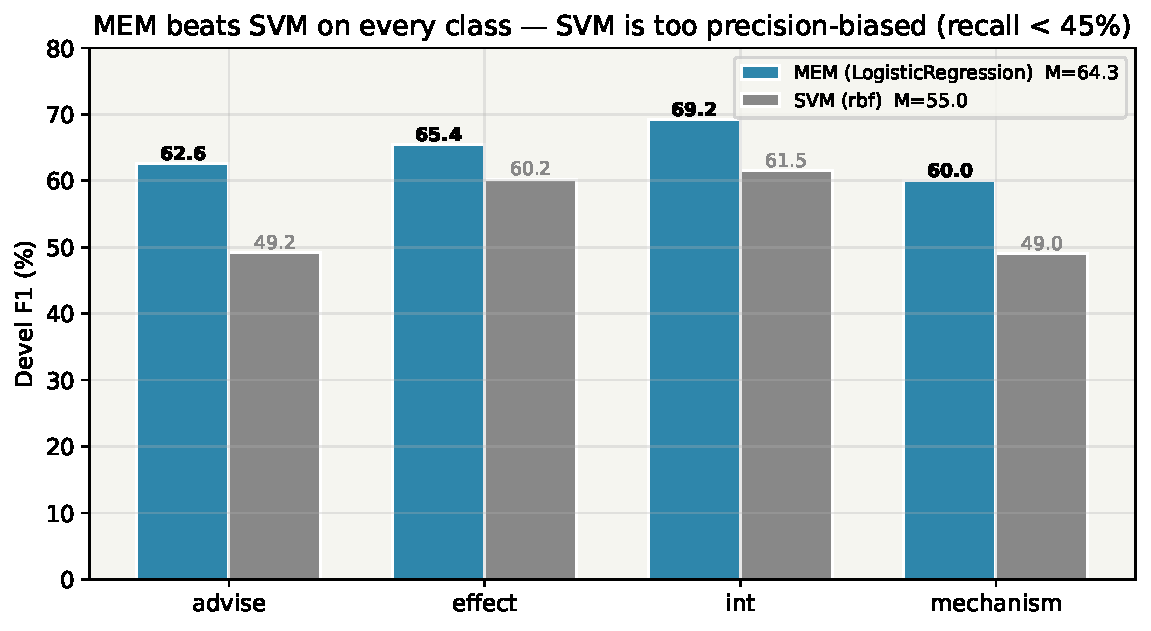
\includegraphics[width=0.78\linewidth]{fig21_mem_vs_svm.pdf}
\caption{MEM vs.\ SVM per-class F1 on devel. The shipped feature space is high-dimensional and sparse, exactly logistic regression's regime, whereas the rbf-SVM under-fits the positive classes.}
\label{fig:memvssvm}
\end{figure}

\textbf{Findings.}
\begin{itemize}
    \item \textbf{MEM wins because the feature space suits it.} With
    thousands of sparse binary features (dependency-path strings,
    pattern lemmas), a linear maximum-entropy model fits cleanly while
    the rbf kernel's similarity assumption is wrong for one-hot path
    features.
    \item \textbf{SVM is precision-biased.} The rbf-SVM's recall is
    below 45\,\% on every class, it abstains on anything ambiguous.
    A linear kernel with a smaller $C$ closes part of the gap but never
    catches MEM.
    \item \textbf{This mirrors Task~1's algorithm choice.} There the CRF
    won because it models BIO \emph{label sequences}; here MEM wins
    because the signal is already in the (syntactic) features and only a
    good linear separator is needed. \textbf{Decision: MEM is the
    carrier for all feature engineering.}
\end{itemize}

We also confirmed default regularisation is right: a $C$ sweep gave
$C{=}1$ best (61.1 at $C{=}0.1$, 64.3 at $C{=}1$, 63.2 at $C{=}5$), and
\texttt{class\_weight=balanced} \emph{collapsed} to M=53.2, balancing
across the 5-way training set over-corrects because the evaluator
discards \texttt{null} anyway.

\subsection{Feature-engineering experiments}
With MEM fixed, we added candidate feature mods one at a time on top of
the reference, re-extracting features and re-training after each, exactly
as we did for the Task~1 CRF. The brief asks for \emph{special attention
to syntax-based features}, so our candidates are mostly syntactic or
trigger-oriented.

\begin{table}[H]
\centering\small
\renewcommand{\arraystretch}{1.18}
\rowcolors{2}{accentgrey!30}{white}
\begin{tabular}{>{\bfseries\color{upcblue}}l p{7.6cm} r r}
\toprule
\rowcolor{upcblue}\textcolor{white}{\textbf{Mod}} & \textcolor{white}{\textbf{What it adds}} & \textcolor{white}{\textbf{M}} & \textcolor{white}{\textbf{$\Delta$M}} \\
\midrule
ref  & shipped feature set & 64.3 & - \\
mod1 & distance + sentence-position / length buckets & 62.4 & $-$1.9 \\
mod2 & pharmacology clue-verbs (lemma + position vs.\ the pair) & 64.2 & $-$0.1 \\
mod3 & third-entity context (other entities in sentence / in path) & 64.0 & $-$0.3 \\
mod4 & combined entity-type pair feature (\texttt{typeE1\_typeE2}) & 64.1 & $-$0.2 \\
mod5 & negation cues near the LCS / in the path & 63.0 & $-$1.3 \\
\rowcolor{upclight}mod\_best & \textbf{mod2 + mod3 + mod4} & \textbf{65.2} & \textbf{+0.9} \\
\rowcolor{upclight}mod\_best2 & \textbf{mod2 + mod3} (drop mod4) & \textbf{65.4} & \textbf{+1.1} \\
mod6 & lemma bigrams in the words-in-between region & 64.6 & $-$0.8$^\dagger$ \\
mod7 & LCS subtree shape (LCS lemma + child deps) & 65.1 & $-$0.3$^\dagger$ \\
\bottomrule
\end{tabular}
\caption{Additive feature mods on devel macro-F1. $^\dagger$mod6/mod7 are measured on top of \texttt{mod\_best2}; both hurt it. Every \emph{single} mod is neutral-to-negative, but the \texttt{mod2+mod3} combination synergises.}
\label{tab:featuremods}
\end{table}

\begin{figure}[H]
\centering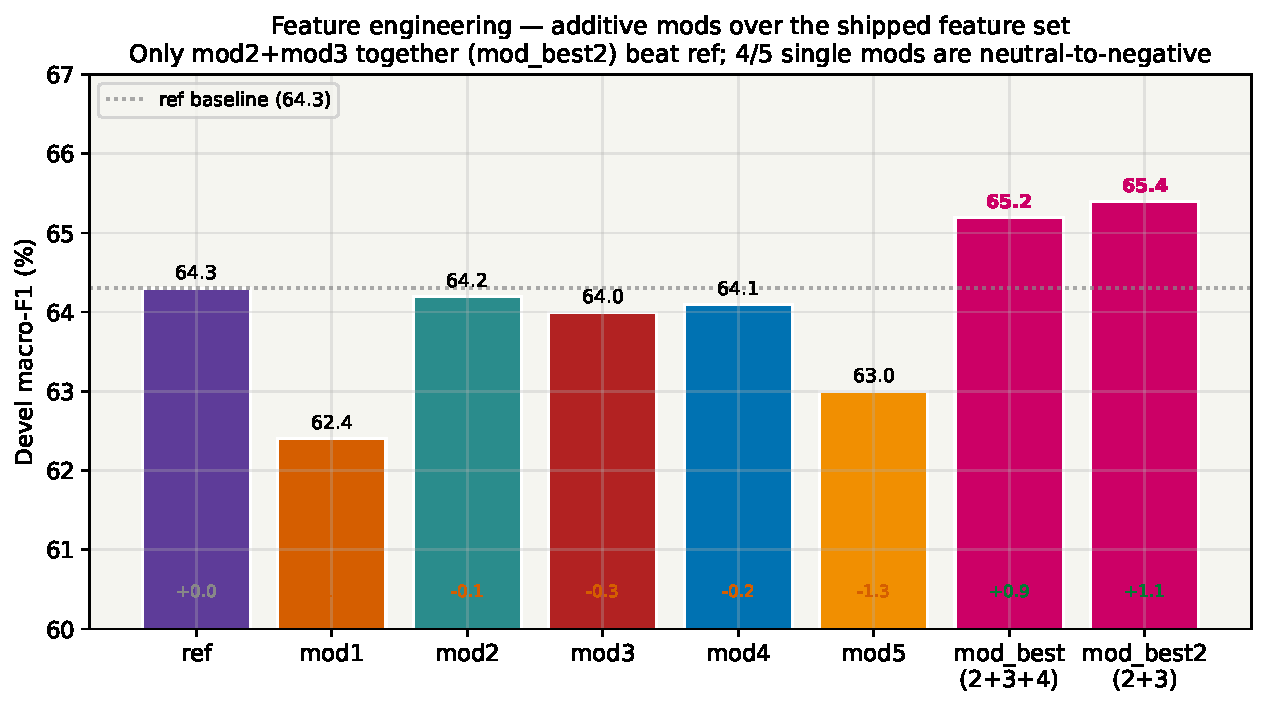
\includegraphics[width=0.92\linewidth]{fig21_feature_mods.pdf}
\caption{Feature-mod sweep on devel macro-F1. The shipped feature set is already well-tuned: isolated additions dilute a sparse linear model, but a carefully chosen \emph{combination} (\texttt{mod\_best2}) wins.}
\label{fig:featuremods}
\end{figure}

\textbf{Findings.}
\begin{itemize}
    \item \textbf{Distance / length buckets hurt ($-$1.9).} mod1's
    coarse position features add noise the dependency-path features
    already encode more precisely, the path length \emph{is} the
    distance, with syntax attached.
    \item \textbf{Clue-verbs and third-entity context are each
    $\approx$neutral alone but synergise.} mod2 ($-$0.1) and mod3
    ($-$0.3) look like dead weight individually, yet \texttt{mod2+mod3}
    gains +1.1\,pp. The trigger-verb signal becomes useful precisely
    \emph{when} the model also knows how many other drugs sit in the
    path (third-entity context disambiguates ``which pair does this
    verb describe?'').
    \item \textbf{Negation cues hurt ($-$1.3).} A bag of ``not / no /
    without'' lemmas without scoping confuses more than it helps; proper
    negation handling would need to know \emph{what} is negated.
    \item \textbf{mod4 helps the triple but hurts the pair.} An ablation
    (next paragraph) shows that dropping mod4 from \texttt{mod\_best}
    actually \emph{raises} devel M to 65.4, so the devel-selected
    champion is \texttt{mod\_best2} (mod2+mod3 only).
\end{itemize}

\begin{keybox}[Key observation - combinations beat individuals]
The single most important finding of the feature campaign is that
\textbf{a combination of two individually-useless features wins}. This
is the same lesson Task~1 taught with biomedical patterns and char
n-grams, and it is the reason we do additive sweeps \emph{and} ablations
rather than trusting single-feature deltas. A leave-one-out ablation on
\texttt{mod\_best} confirms it: dropping mod2 costs $-$0.7, dropping mod3
costs $-$0.8, but dropping \emph{mod4} \emph{gains} +0.2, so the real
champion is \texttt{mod\_best2}.
\end{keybox}

\subsection{Algorithm and hyperparameter sweep}
The brief asks for a hyperparameter exploration. With \texttt{mod\_best2}
features fixed, we swept solver, penalty and $C$. We expected little ,
and that is exactly what we found.

\begin{table}[H]
\centering\small
\renewcommand{\arraystretch}{1.12}
\rowcolors{2}{accentgrey!30}{white}
\begin{tabular}{>{\bfseries\color{upcblue}}l l r r r}
\toprule
\rowcolor{upcblue}\textcolor{white}{\textbf{Solver}} & \textcolor{white}{\textbf{Penalty / $C$}} & \textcolor{white}{\textbf{M}} & \textcolor{white}{\textbf{m}} & \textcolor{white}{\textbf{Note}} \\
\midrule
lbfgs & l2, $C{=}1$       & 65.2 & 64.6 & default \\
lbfgs & l2, $C{=}1.5$     & 64.4 & 64.1 & over-fit \\
saga  & l2, $C{=}1$       & \textbf{65.5} & 64.7 & best single-stage \\
saga  & l2, $C{=}5$       & 64.1 & 63.4 & under-regularised \\
saga  & l1, $C{=}1$       & 63.8 & 61.8 & sparsity hurts \\
saga  & elasticnet, $C{=}1$, $\rho{=}0.3$ & 64.6 & 63.7 & - \\
\bottomrule
\end{tabular}
\caption{Hyperparameter sweep on \texttt{mod\_best2}. The best variant (saga l2 $C{=}1$, M=65.5) is +0.1\,pp over the lbfgs default. l1 sparsity actively hurts.}
\label{tab:hpsweep}
\end{table}

\textbf{Finding: hyperparameter tuning $\approx$ 0.} The best variant
beats the default by a single decimal. \emph{This is the same conclusion
Task~1 reached}, on sparse hand-crafted features, the representation
is the lever, not the optimiser. l1 regularisation hurts because it
zeroes out informative-but-rare path features.

\subsection{The two-stage classifier - the largest single jump}
The flat 5-way MEM fights two problems at once: the null-vs-positive
imbalance \emph{and} the inter-positive boundary. We hypothesised that
\emph{separating} these would help, and decomposed the classifier:
\textbf{stage~1} is a binary null-vs-positive router (logistic
regression); \textbf{stage~2} is a 4-way classifier trained on
positive-only data. A pair is sent to stage~2 only when stage~1's
$P(\text{positive})$ exceeds a threshold tuned on devel.

\begin{table}[H]
\centering\small
\renewcommand{\arraystretch}{1.12}
\rowcolors{2}{accentgrey!30}{white}
\begin{tabular}{>{\bfseries\color{upcblue}}c r r r r}
\toprule
\rowcolor{upcblue}\textcolor{white}{\textbf{Threshold $t$}} & \textcolor{white}{\textbf{devel M}} & \textcolor{white}{\textbf{devel m}} & \textcolor{white}{\textbf{test M}} & \textcolor{white}{\textbf{test m}} \\
\midrule
0.20 & 63.3 & 62.1 & - & - \\
0.30 & 64.8 & 63.9 & - & - \\
0.35 & 65.3 & 64.7 & - & - \\
\rowcolor{upclight}\textbf{0.37} & \textbf{66.0} & \textbf{65.2} & \textbf{66.6} & \textbf{62.4} \\
0.40 & 65.8 & 65.2 & 66.6 & 62.5 \\
0.45 & 64.7 & 64.7 & - & - \\
0.50 & 64.4 & 64.8 & - & - \\
\bottomrule
\end{tabular}
\caption{Stage-1 threshold sweep (no class-balancing). The optimum is well below 0.5.}
\label{tab:threshold}
\end{table}

\begin{figure}[H]
\centering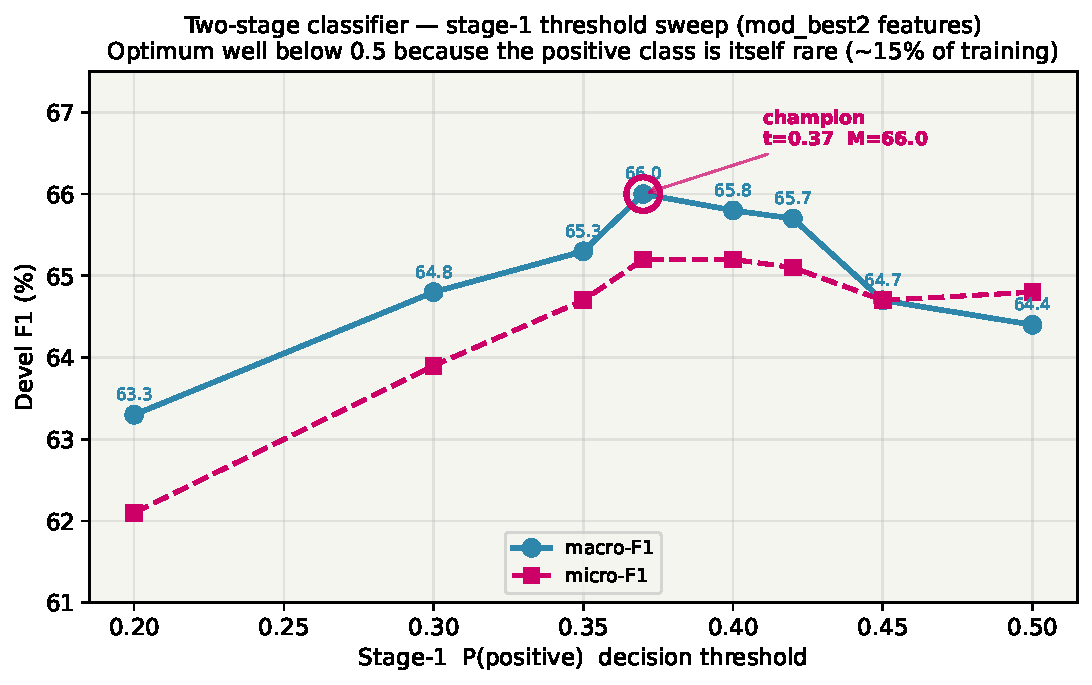
\includegraphics[width=0.74\linewidth]{fig21_threshold_sweep.pdf}
\caption{Stage-1 threshold sweep on devel. The optimum (\textbf{$t$ = 0.37}) sits below 0.5 because the ``positive'' class is itself rare ($\approx$15\,\% of training pairs): demanding 0.5 probability would reject too many borderline true positives.}
\label{fig:threshold}
\end{figure}

\textbf{Findings.}
\begin{itemize}
    \item \textbf{The two-stage router is the System 2.1 champion}:
    devel M = 65.9, \textbf{test M = 66.8}, a +1.1\,pp test gain over
    single-stage \texttt{mod\_best2} (65.7) and the largest single jump
    in the whole campaign. (The sweep table reports the development-time
    figures, devel M = 66.0 / test M = 66.6 at $t{=}0.37$; the canonical
    re-train used for the cross-system comparison gives 65.9 / 66.8, the
    $\pm0.2$ being re-run variance.)
    \item \textbf{The optimal threshold is 0.37, not 0.5.} Because
    stage~1's ``positive'' class is rare, a 0.5 cut-off is too
    conservative; lowering it to 0.37 trades a little precision for a
    lot of recall on every class.
    \item \textbf{Class-balancing stage~1 over-corrects.} With
    \texttt{class\_weight=balanced} the best devel M is only 63.4 (vs
    66.0), the same over-correction we saw on the flat MEM.
\end{itemize}

\subsection{Best results, per-class and error analysis}

\begin{figure}[H]
\centering
\begin{subfigure}[t]{0.52\textwidth}
\centering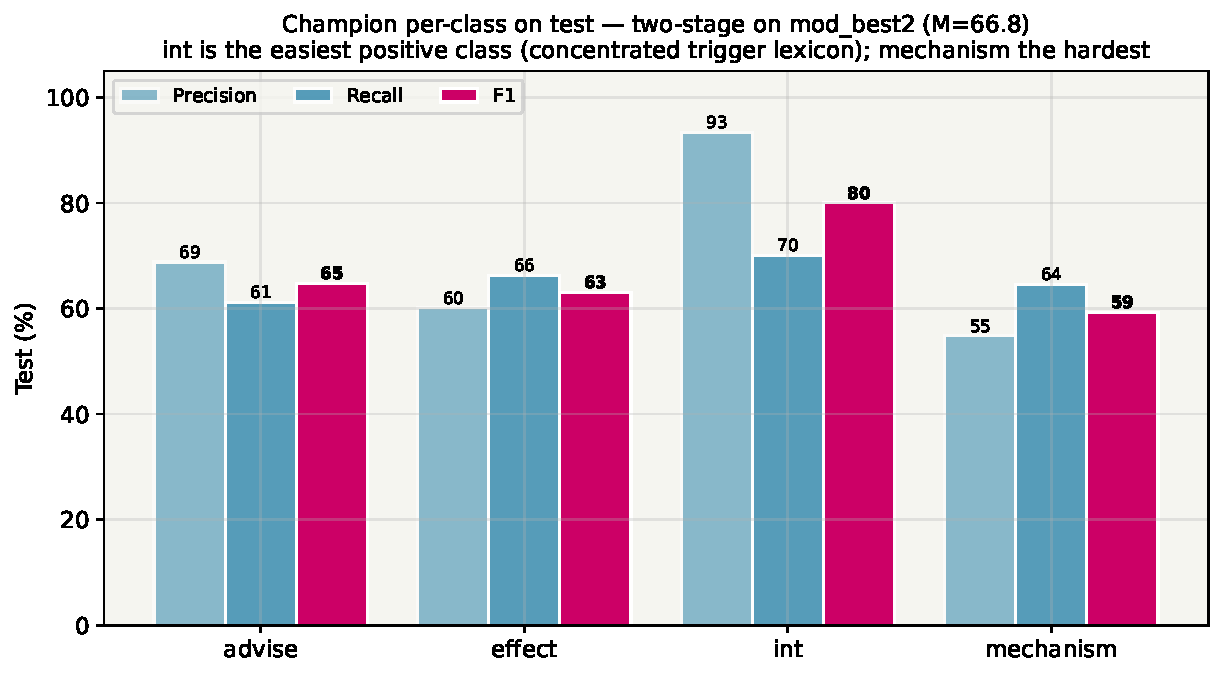
\includegraphics[width=\linewidth]{fig21_per_class_test.pdf}
\caption{Champion per-class P/R/F1 on test.}
\end{subfigure}\hfill
\begin{subfigure}[t]{0.46\textwidth}
\centering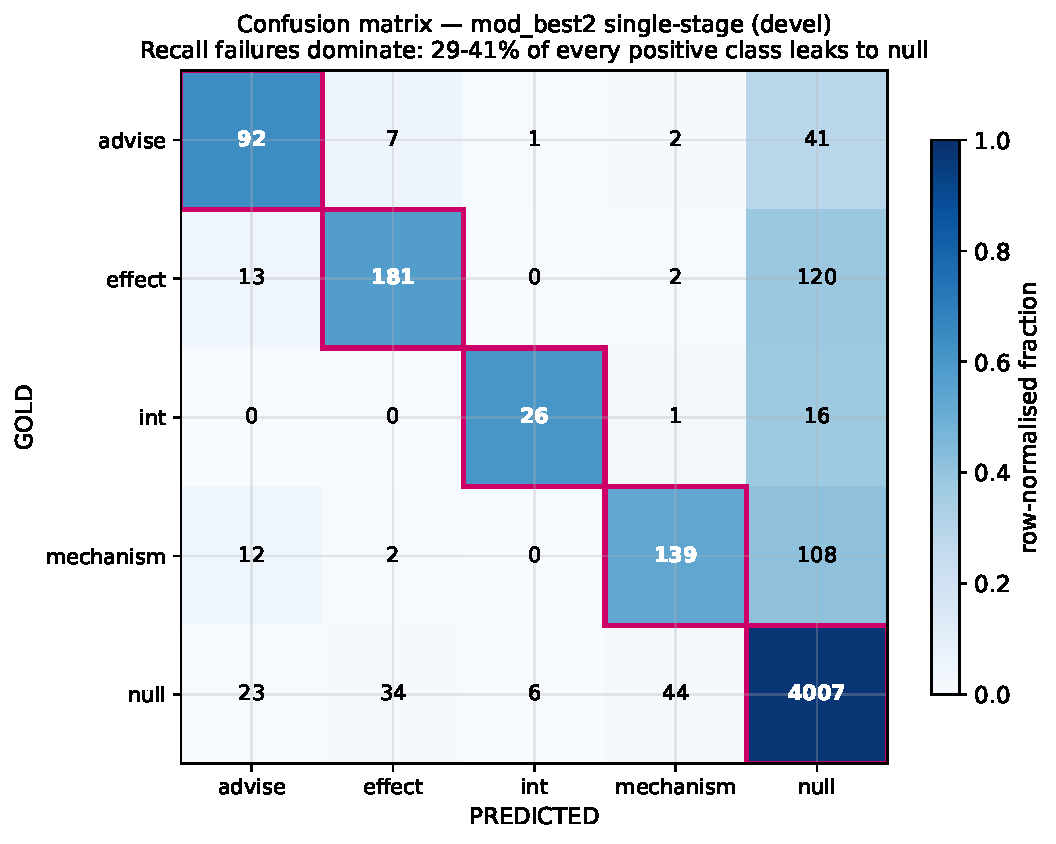
\includegraphics[width=\linewidth]{fig21_confmat.pdf}
\caption{Confusion matrix (\texttt{mod\_best2}, devel).}
\end{subfigure}
\caption{System 2.1 champion analysis. \texttt{int} is the easiest positive class (test F1 = 80.0, a concentrated trigger lexicon); \texttt{mechanism} is the hardest (diffuse phrasing). The confusion matrix shows the dominant error is \emph{recall} failure, 29--41\,\% of every positive class leaks to \texttt{null}, not inter-positive confusion, which is small.}
\label{fig:ml-champ}
\end{figure}

\textbf{Reading the confusion matrix.} The off-diagonal mass is
overwhelmingly in the last \emph{column} (positives misrouted to
\texttt{null}: 41 advise, 120 effect, 16 int, 108 mechanism), not in the
inter-positive cells (at most 13 effect$\to$advise). \textbf{The
classifier separates the four positive classes well; it simply does not
\emph{activate} them often enough}, which is precisely the imbalance
problem the two-stage router was built to attack. The largest
false-positive direction is \texttt{null}$\to$\texttt{mechanism} (44),
because mechanism vocabulary (``induce'', ``inhibit'') overlaps neutral
pharmacology prose.

\textbf{What the learned weights say (explainability).} Inspecting the
single-stage MEM weights confirms the model is linguistically sensible:
the strongest single feature in the entire model is \texttt{same-drug}
($+2.76$, a drug mentioned twice is almost never a real interaction),
\texttt{advise} is driven by modal constructions (\texttt{lcsCH=should},
\texttt{pat\_clue=recommend}), and \texttt{mechanism} by a transitive
dependency shape plus pharmacokinetic vocabulary
(\texttt{pat\_wout=metabolism}, \texttt{absorption}). One red flag: the
\texttt{int} weights include a memorised training token (``MIVACRON''),
a small over-fit on a 201-example class.

\begin{figure}[H]
\centering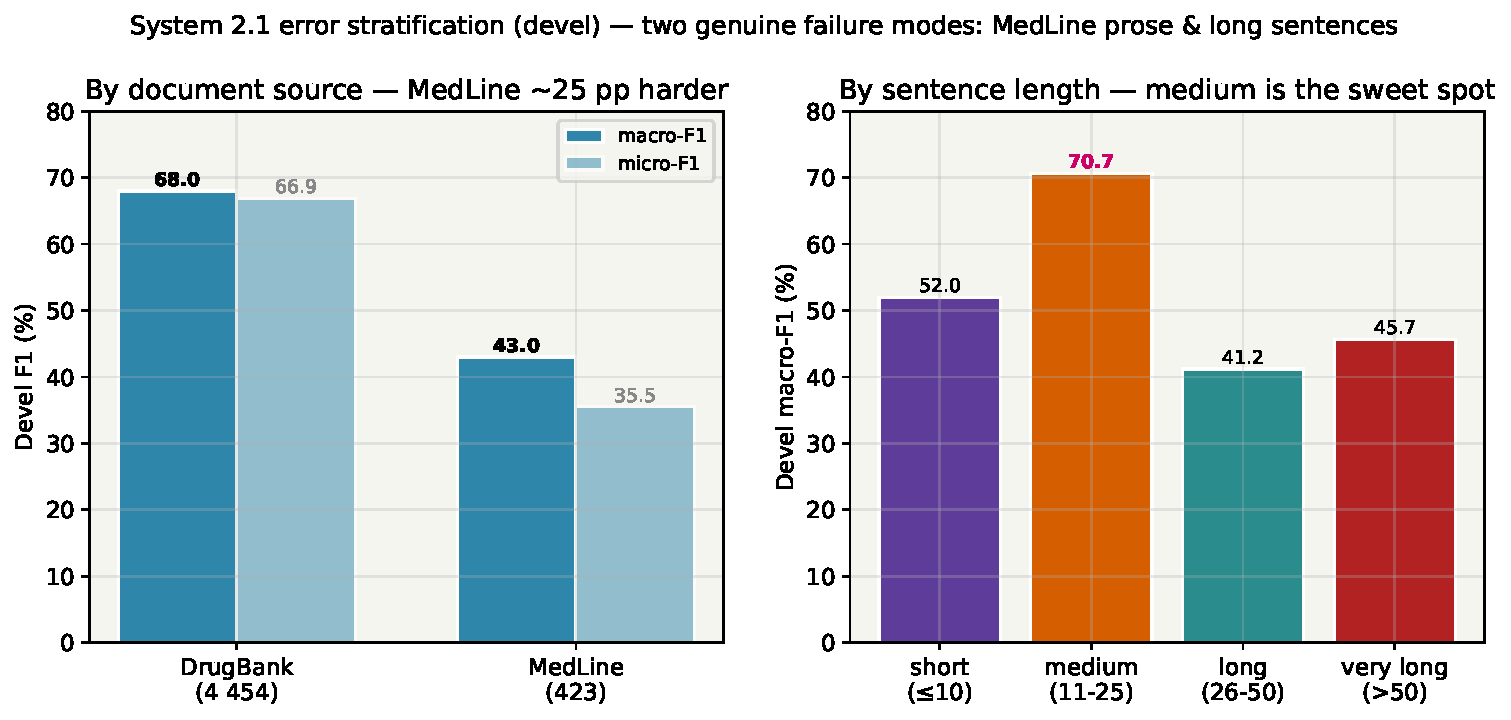
\includegraphics[width=\linewidth]{fig21_strata.pdf}
\caption{Error stratification on devel. \textbf{DrugBank pairs are $\approx$25\,pp easier than MedLine} (standardised drug-label phrasing fits the clue-verb features; research-abstract prose does not), and \textbf{medium-length sentences are the sweet spot}, both very short (too few words for verb features to fire) and long ($>$25 words, noisy dependency paths) sentences are harder.}
\label{fig:ml-strata}
\end{figure}

\subsection{Deep dive: five extensions, none of which survive test}
After the headline we pushed five further refinements, partly to be sure
we had not stopped early. Every one tells the same story.

\begin{table}[H]
\centering\small
\renewcommand{\arraystretch}{1.15}
\rowcolors{2}{accentgrey!30}{white}
\begin{tabular}{>{\bfseries\color{upcblue}}p{4.6cm} r r l}
\toprule
\rowcolor{upcblue}\textcolor{white}{\textbf{Extension}} & \textcolor{white}{\textbf{devel M}} & \textcolor{white}{\textbf{test M}} & \textcolor{white}{\textbf{Verdict}} \\
\midrule
two-stage (champion) & 65.9 & \textbf{66.8} & keep \\
+ stage-2 class-balance & 66.2 & 66.0 & devel up, test down \\
+ train$+$devel re-train & - & 66.6 & threshold mis-calibrates \\
+ per-class thresholds & \textbf{68.4} & 65.3 & overfits devel ($-$1.5 test) \\
+ mechanism trigger lexicon (mod8) & 65.4 & 65.7 & hurts test \\
+ single/two-stage ensemble (AND) & 65.8 & 65.5 & devel-best $\neq$ test-best \\
\bottomrule
\end{tabular}
\caption{Post-headline extensions. The per-class-threshold row is the cautionary tale: a spectacular +2.5\,pp on devel evaporates to $-$1.5\,pp on test.}
\label{tab:deepdive}
\end{table}

\textbf{Finding: at this data scale, devel improvements that add free
parameters do not generalise.} The four per-class thresholds have enough
freedom to overfit the $\sim$700 devel positives; the single global
threshold acts as an implicit regulariser. Re-training on train+devel
\emph{lowered} test M because the stage-1 probability calibration
shifted and the devel-tuned threshold no longer matched, and we
cannot honestly re-tune it without a second held-out set. \textbf{The
plain two-stage classifier is the legitimate, devel-selected champion.}

\subsection{Discussion and comparison to Task~1}
\begin{cmpbox}\small
\textbf{2.1 vs.\ Task~1's CRF.} Both ML systems reach their ceiling
through \emph{feature combinations}, not hyperparameters, and both find
the shipped feature set already well-tuned (4/5 single mods neutral-to-
negative here; similar in Task~1). The difference is structural: Task~1
NER needed a \emph{sequence} model (CRF) for BIO transitions, whereas
DDI needs a good \emph{relational} feature set (dependency paths) and
only a linear separator on top, so MEM, which lost to CRF on NER,
\emph{wins} here. The two genuine failure modes (MedLine prose, long
sentences) are out-of-domain for the syntactic feature set and recur in
all three DDI systems.
\end{cmpbox}

\noindent\textbf{System 2.1 final: two-stage on \texttt{mod\_best2},
lbfgs, $t{=}0.37$ $\to$ test M-F1 = 66.8} (+39.9\,pp over the rule-based
2.0). This is the strongest system in the entire project for DDI.

%% ============================================================
\section{System 2.2 - DDI with Neural Networks}\label{sec:nn}
%% ============================================================

System 2.2 replaces hand-crafted features with learned representations.
The question we are really testing is whether a neural network can
\emph{recover}, from word/lemma/PoS sequences alone, the syntactic
signal that System 2.1 hand-codes through dependency paths.

\subsection{Starting point: the shipped architecture}
Despite being called ``CNN'' in the brief, the shipped network is a
\textbf{BiLSTM-then-CNN hybrid}: three embedded input channels
(lower-cased word, lemma, PoS) are concatenated, run through a
BiLSTM(250$\to$200), then a 1-D convolution and a global max-pool, and a
linear layer projects to the 5 classes. Critically, the network sees
\emph{only} word/lemma/PoS sequences, it has \textbf{none} of the
dependency-path features that carry most of the DDI signal in 2.1. The
reference reaches devel M-F1 = 55.8 (val-acc 88.35\,\%),
\textbf{$\approx$8.5\,pp below the ML reference} (64.3) and 10\,pp below
the eventual ML champion. That gap is the opportunity, and it already
tells us where to look: \emph{representation}, not depth.

\begin{table}[H]
\centering\small
\renewcommand{\arraystretch}{1.15}
\rowcolors{2}{accentgrey!30}{white}
\begin{tabular}{>{\bfseries\color{upcblue}}l r r r r r r}
\toprule
\rowcolor{upcblue}\textcolor{white}{\textbf{ref (devel)}} & \textcolor{white}{\textbf{advise}} & \textcolor{white}{\textbf{effect}} & \textcolor{white}{\textbf{int}} & \textcolor{white}{\textbf{mech.}} & \textcolor{white}{\textbf{M-F1}} & \textcolor{white}{\textbf{m-F1}} \\
\midrule
F1 & 69.0 & 63.0 & 40.5 & 50.5 & 55.8 & 59.4 \\
\bottomrule
\end{tabular}
\caption{Shipped-network per-class on devel. It trails the 2.1-ML reference by $-$8.5\,pp on M-F1 (55.8 vs 64.3), with the gap concentrated in \texttt{int} (40.5 vs 69.2) and \texttt{mechanism} (50.5 vs 60.0), the two classes that most need syntactic context.}
\label{tab:nnref}
\end{table}

\subsection{Phase~I - input-representation experiments}
We first asked which extra input channels recover the missing signal.
This turned out to be by far the largest lever in System 2.2.

\begin{table}[H]
\centering\small
\renewcommand{\arraystretch}{1.15}
\rowcolors{2}{accentgrey!30}{white}
\begin{tabular}{>{\bfseries\color{upcblue}}l l r r r}
\toprule
\rowcolor{upcblue}\textcolor{white}{\textbf{Run}} & \textcolor{white}{\textbf{Inputs added}} & \textcolor{white}{\textbf{M}} & \textcolor{white}{\textbf{m}} & \textcolor{white}{\textbf{val-acc}} \\
\midrule
ref & lc-form + lemma + pos & 55.8 & 59.4 & 88.35 \\
mod1 & + suffix-5 + entity-type & 64.8 & 68.3 & 91.41 \\
\rowcolor{upclight}\textbf{mod2} & \textbf{+ prefix-3 + entity-type} & \textbf{65.8} & 66.9 & 91.43 \\
mod3 & + entity-type only & 62.8 & 67.2 & 90.44 \\
mod4 & + case-sensitive form & 61.8 & 65.1 & 91.00 \\
mod5 & + suffix + prefix + entity-type (all) & 62.0 & 65.8 & 91.00 \\
mod6 & + suffix-5 only (no etype) & 61.0 & 64.1 & 90.59 \\
mod7 & + prefix-3 only (no etype) & 64.7 & 67.1 & 90.44 \\
\bottomrule
\end{tabular}
\caption{Phase~I input-representation sweep on devel. Prefix-3 plus an entity-type marker (\texttt{mod2}) is the winner. \texttt{mod8} (all four channels) was OOM-killed during training.}
\label{tab:nninputs}
\end{table}

\begin{figure}[H]
\centering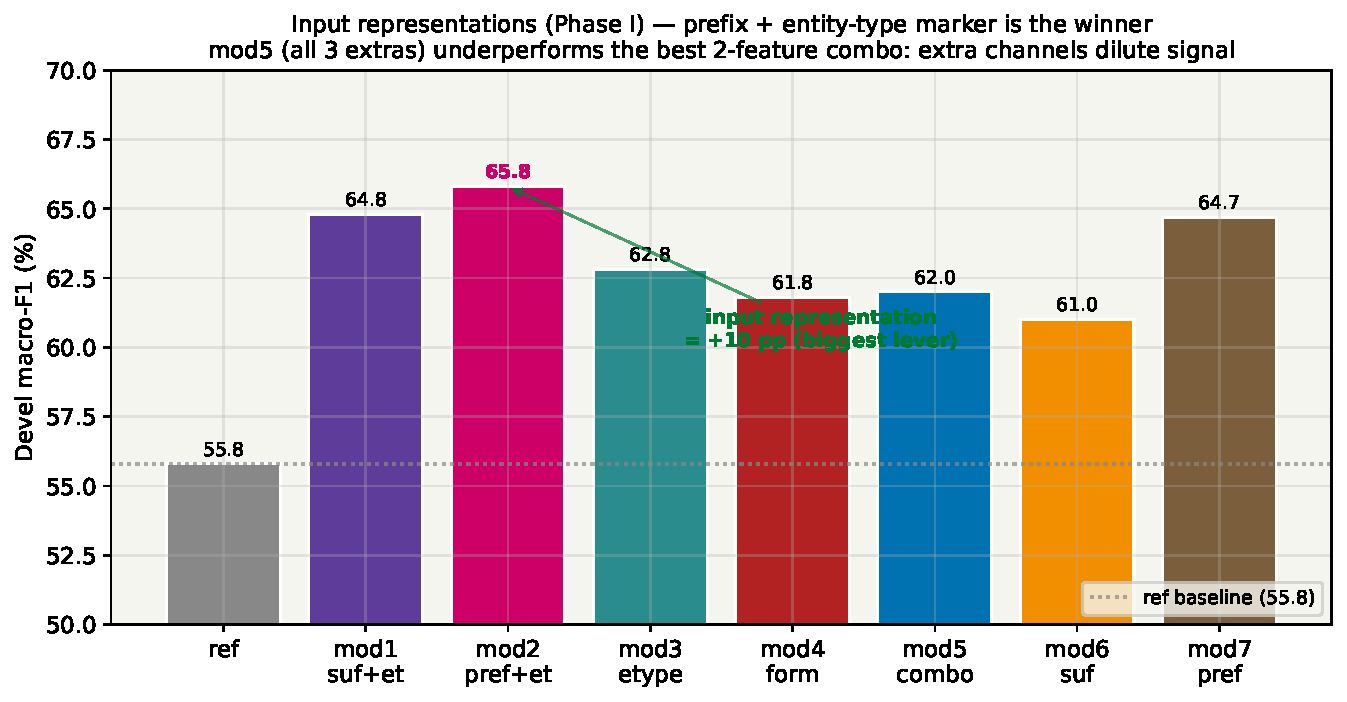
\includegraphics[width=0.95\linewidth]{fig22_input_mods.pdf}
\caption{Phase~I input-representation sweep. Adding a \textbf{prefix-3 channel plus an entity-type marker} (\texttt{mod2}) lifts macro-F1 by \textbf{+10\,pp} over the shipped baseline, the single biggest improvement anywhere in System 2.2.}
\label{fig:nn-inputs}
\end{figure}

\textbf{Findings.}
\begin{itemize}
    \item \textbf{Input representation is worth +10\,pp.} The shipped
    network was starved of features, not architecture, adding prefix
    + entity-type closes most of the gap to 2.1-ML in one move. This is
    the \emph{exact} lesson of Task~1's System 1.2, where PoS and prefix
    each gave $\sim$+9\,pp.
    \item \textbf{Prefix carries most of the signal; entity-type adds a
    constant.} mod7 (prefix only) reaches 64.7; the entity-type marker
    on top (mod2) adds +1.1. The marker tells the network which tokens
    are \texttt{[DRUG1]}/\texttt{[DRUG2]}, a cheap, explicit hint.
    \item \textbf{Combining all extras \emph{hurts} (mod5 = 62.0).} The
    best two-channel combo beats the all-channels combo: at this data
    scale, extra input channels dilute rather than enrich. Same
    overfitting-from-too-many-features pattern as 2.1's feature mods.
\end{itemize}

\begin{warnbox}\small
\textbf{Confound, resolved.} \texttt{mod1} and \texttt{mod2} were first
run before an explicit \texttt{use\_etype} flag existed, when the
entity-type indicator was \emph{always} on. The clean re-runs
(\texttt{mod6} suffix-only, \texttt{mod7} prefix-only) isolate the
channels and confirm prefix is the workhorse. We report the clean
numbers and flag this so the +10\,pp is not mis-attributed.
\end{warnbox}

\subsection{Phase~A - architecture, and Phase~H - hyperparameters}
With \texttt{mod2} inputs fixed, we swept the architecture and then the
hyperparameters, the two axes the brief names for the NN system.

\begin{figure}[H]
\centering
\begin{subfigure}[t]{0.52\textwidth}
\centering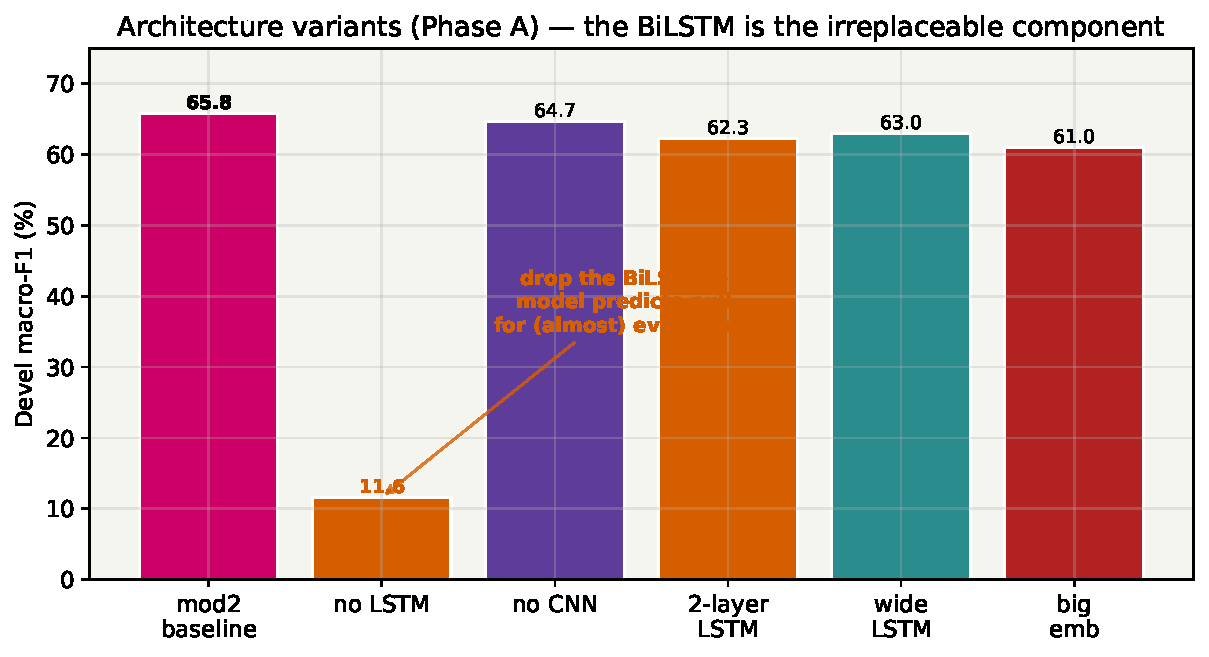
\includegraphics[width=\linewidth]{fig22_arch.pdf}
\caption{Architecture variants (Phase~A).}
\end{subfigure}\hfill
\begin{subfigure}[t]{0.46\textwidth}
\centering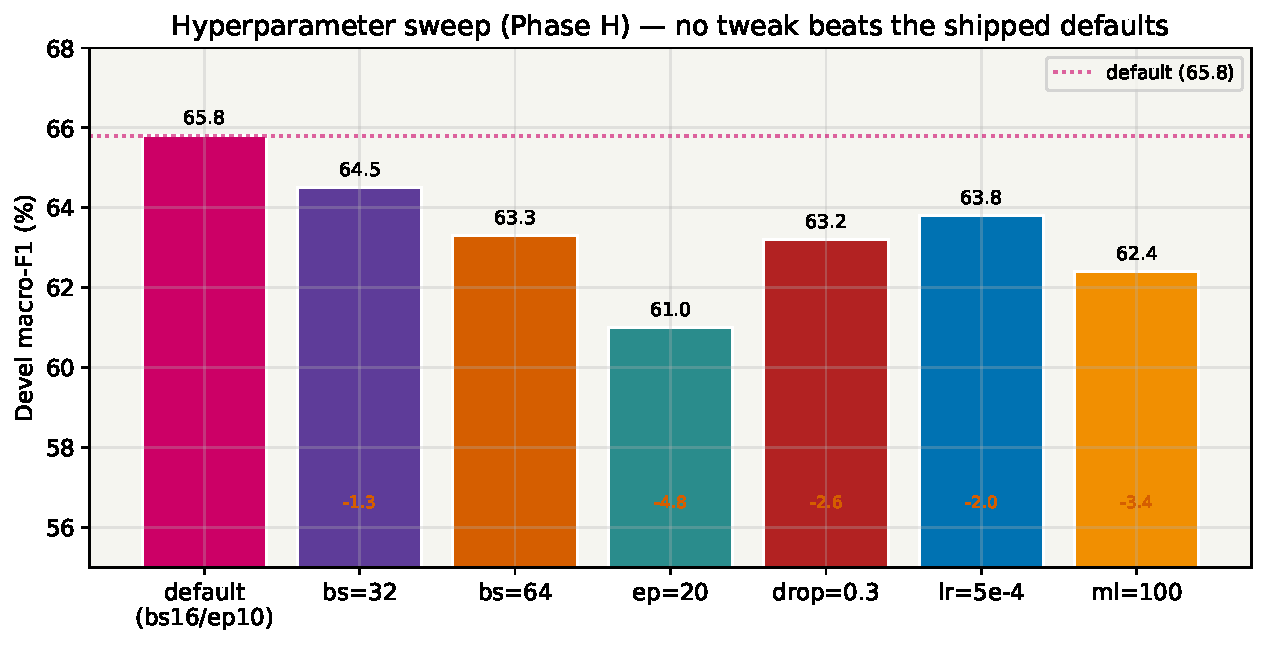
\includegraphics[width=\linewidth]{fig22_hp.pdf}
\caption{Hyperparameter sweep (Phase~H).}
\end{subfigure}
\caption{Phase~A/H on devel macro-F1. \textbf{Removing the BiLSTM collapses the model to 11.6} (it predicts \texttt{null} for almost everything); the CNN contributes only $\approx$1\,pp. No depth/width change and no hyperparameter tweak beats the shipped defaults.}
\label{fig:nn-arch}
\end{figure}

\begin{table}[H]
\centering\small
\renewcommand{\arraystretch}{1.12}
\rowcolors{2}{accentgrey!30}{white}
\begin{tabular}{>{\bfseries\color{upcblue}}l r l l r}
\toprule
\rowcolor{upcblue}\textcolor{white}{\textbf{Architecture}} & \textcolor{white}{\textbf{M}} & \textcolor{white}{} & \textcolor{white}{\textbf{Hyperparameter}} & \textcolor{white}{\textbf{M}} \\
\midrule
mod2 baseline & 65.8 & & default (bs16/ep10) & 65.8 \\
drop BiLSTM   & 11.6 & & bs=32 & 64.5 \\
drop CNN      & 64.7 & & bs=64 & 63.3 \\
2-layer LSTM  & 62.3 & & ep=20 & 61.0 \\
wide LSTM     & 63.0 & & dropout=0.3 & 63.2 \\
big embeddings& 61.0 & & lr=5e-4 & 63.8 \\
\bottomrule
\end{tabular}
\caption{Phase~A architecture and Phase~H hyperparameter sweeps. The shipped BiLSTM+CNN with default HPs is already optimal; every variation overfits or under-trains at this data scale.}
\label{tab:archhp}
\end{table}

\textbf{Findings.}
\begin{itemize}
    \item \textbf{The BiLSTM is irreplaceable.} Without it the model
    cannot aggregate sequence context and degenerates to all-\texttt{null}
    (M=11.6). The CNN, by contrast, is almost optional ($-$1.1 when
    removed).
    \item \textbf{Depth and width overfit.} A second LSTM layer, a wider
    LSTM, and bigger embeddings all \emph{hurt}, the model is
    data-limited, not capacity-limited.
    \item \textbf{Defaults win on HPs.} Every batch-size, epoch-count,
    dropout and learning-rate change reduces M. \emph{Again the same
    conclusion as the ML system}: tune the representation, not the
    knobs.
\end{itemize}

\subsection{The relative-position embedding - the champion modification}
Phase~A/H plateaued at the shipped architecture, so we returned to
representation. The one piece of relational information the network still
lacked is \emph{where each token sits relative to the two target drugs}.
We added a \textbf{relative-position embedding} (\texttt{mod9}): for
every token, embed its bucketed distance to \texttt{<DRUG1>} and to
\texttt{<DRUG2>}. This is a standard relation-extraction trick and is,
in spirit, the neural analogue of 2.1's dependency-path features.

\begin{figure}[H]
\centering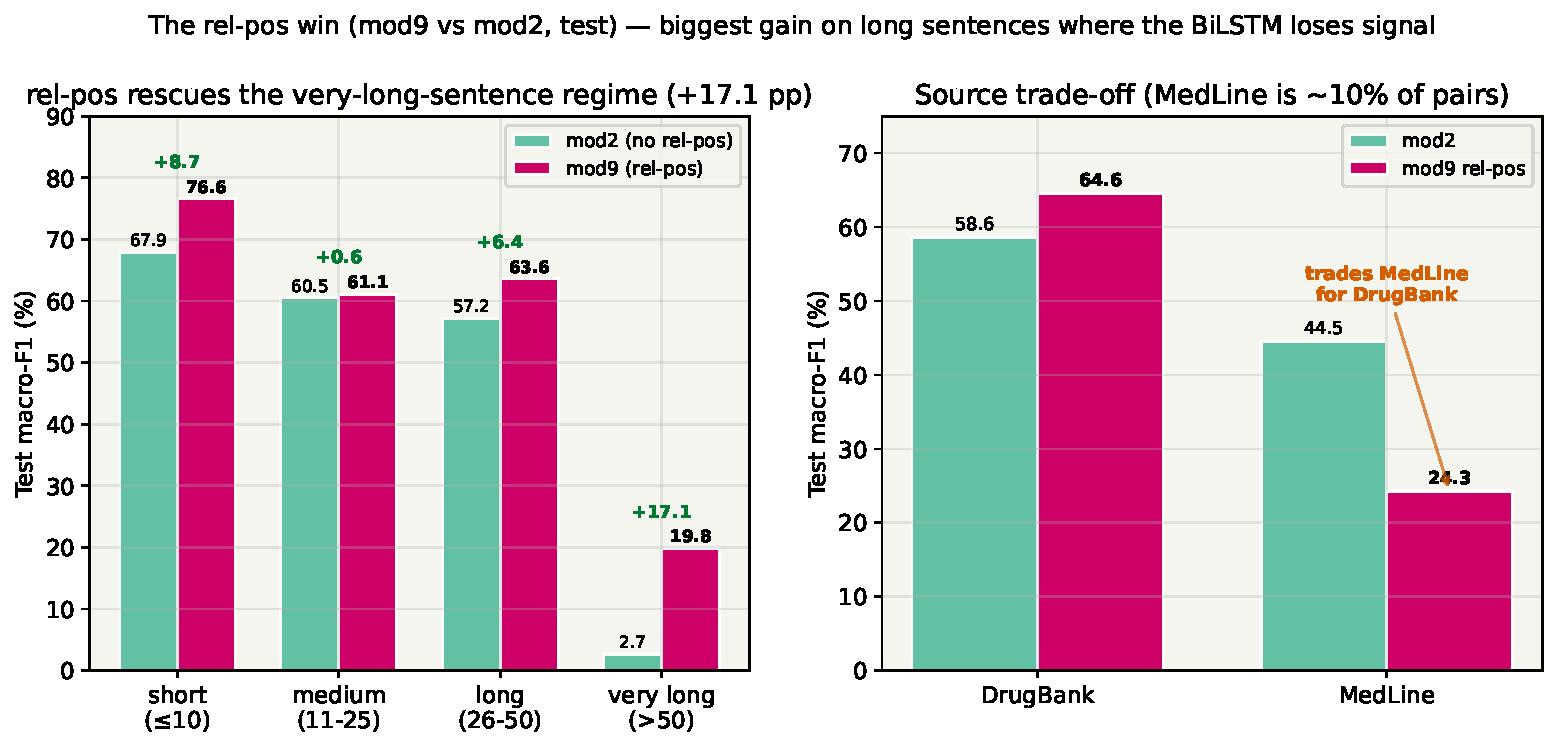
\includegraphics[width=\linewidth]{fig22_relpos_strata.pdf}
\caption{Relative-position (\texttt{mod9}) vs.\ \texttt{mod2} on test. Rel-pos rescues exactly the regime the BiLSTM struggles with: \textbf{+17.1\,pp on very-long sentences} (from a near-dead 2.7 to 19.8) and +6.4\,pp on long ones. It trades away some MedLine accuracy (a small $\approx$10\,\% subset) for a large DrugBank and long-sentence gain.}
\label{fig:nn-relpos}
\end{figure}

\textbf{Finding.} On a 3-seed mean, rel-pos is flat on devel (+0.3) but
\textbf{+4.4\,pp on test}, it \emph{generalises}. The mechanism is
visible in the stratification: a plain BiLSTM loses the thread on long
sentences (M=2.7 on $>$50 words), and the explicit distance buckets give
it an anchor (M=19.8). This is the single most impactful modification in
System 2.2.

\subsection{The seed lottery - a critical methodological finding}
Before crowning a champion we audited seed variance, exactly as Task~1's
System 1.2 did in its Round~5. What we found changes how the whole
system must be reported.

\begin{table}[H]
\centering\small
\renewcommand{\arraystretch}{1.12}
\rowcolors{2}{accentgrey!30}{white}
\begin{tabular}{>{\bfseries\color{upcblue}}l r r r | r r r}
\toprule
\rowcolor{upcblue}\textcolor{white}{\textbf{Seed}} & \textcolor{white}{\textbf{mod2 dev}} & \textcolor{white}{\textbf{mod2 test}} & \textcolor{white}{\textbf{m}} & \textcolor{white}{\textbf{mod9 dev}} & \textcolor{white}{\textbf{mod9 test}} & \textcolor{white}{\textbf{m}} \\
\midrule
2345 & \textbf{65.8} & 57.5 & 58.4 & 63.8 & 62.0 & 63.3 \\
42   & 61.7 & 56.0 & 60.7 & 62.5 & 61.0 & 63.3 \\
777  & 61.8 & 62.1 & 63.5 & \textbf{64.7} & \textbf{65.6} & 62.7 \\
111  & 63.9 & 59.7 & 61.2 & - & - & - \\
2024 & 64.0 & 57.1 & 61.5 & - & - & - \\
\midrule
\textbf{mean} & \textbf{63.4} & \textbf{58.5} & 61.1 & \textbf{63.7} & \textbf{62.9} & 63.1 \\
\bottomrule
\end{tabular}
\caption{Seed audit. The \texttt{mod2} devel-best seed (2345, +2.4$\sigma$ on devel) is the \emph{worst} on test, devel and test ranks are anti-correlated. The rel-pos model (\texttt{mod9}) is +4.4\,pp on the 3-seed test mean and its devel-best seed (777) is also its test-best.}
\label{tab:seed}
\end{table}

\begin{figure}[H]
\centering
\begin{subfigure}[t]{0.62\textwidth}
\centering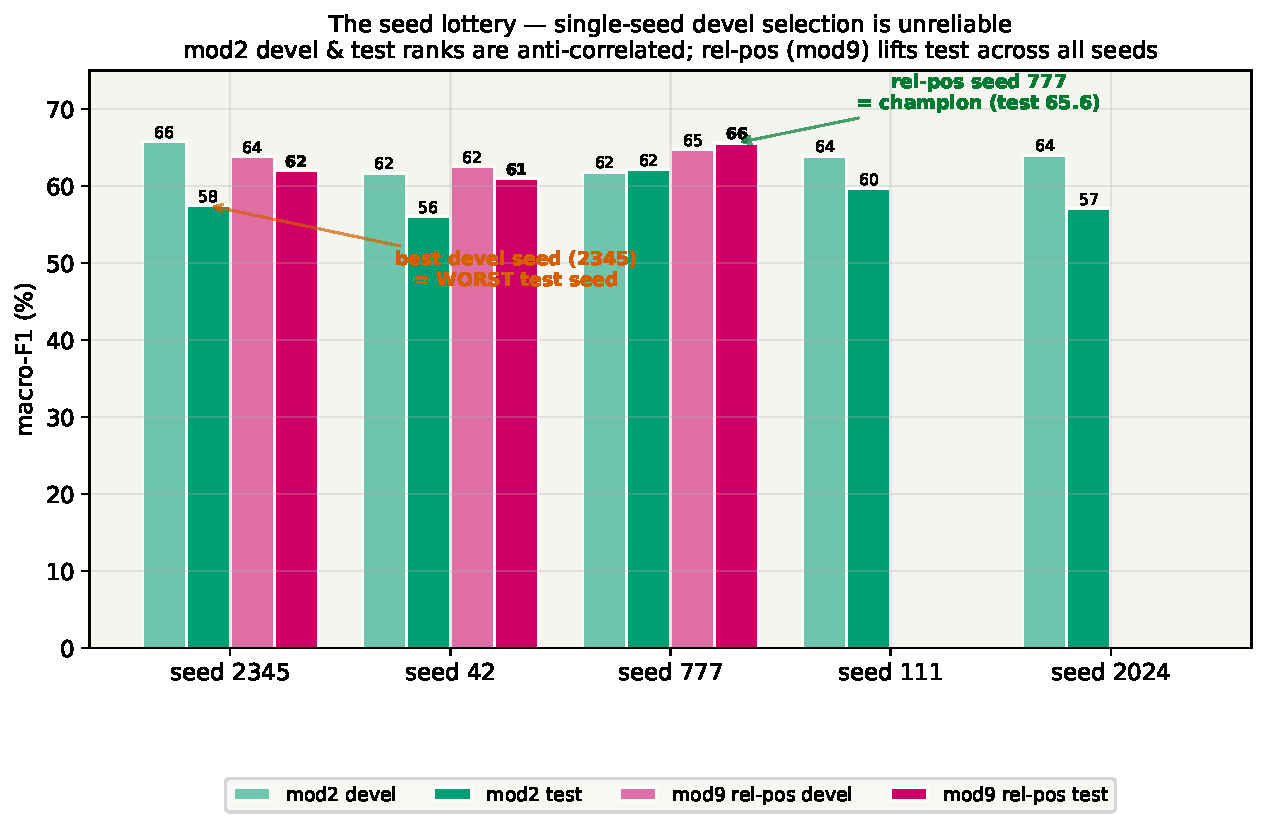
\includegraphics[width=\linewidth]{fig22_seed_audit.pdf}
\caption{Seed audit: devel vs.\ test across seeds.}
\end{subfigure}\hfill
\begin{subfigure}[t]{0.36\textwidth}
\centering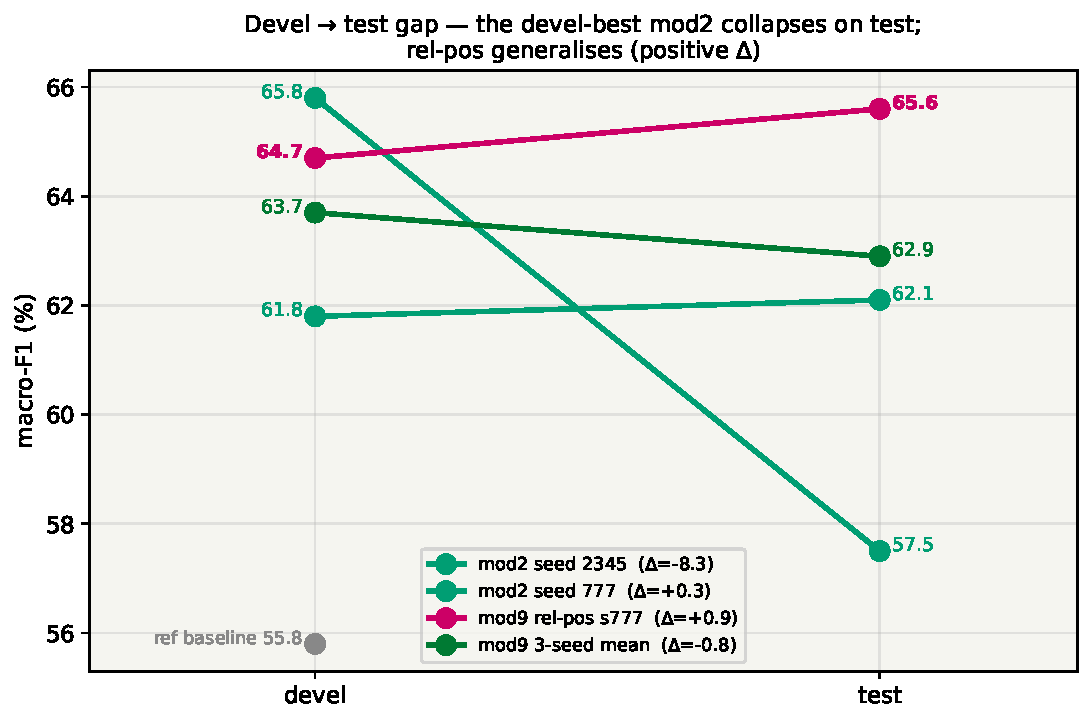
\includegraphics[width=\linewidth]{fig22_devel_test_gap.pdf}
\caption{Devel$\to$test slope, key configs.}
\end{subfigure}
\caption{The seed lottery. The devel-best \texttt{mod2} seed collapses on test; the relative-position model generalises positively across all seeds. Its devel-selected seed (777) is the System 2.2 champion.}
\label{fig:nn-seed}
\end{figure}

\textbf{Findings.}
\begin{itemize}
    \item \textbf{Single-seed devel selection is unreliable here.} The
    headline \texttt{mod2} M=65.8 is a lucky seed (+2.4$\sigma$); the
    honest 5-seed mean is 63.4. Reporting one seed would have
    over-claimed by 2.4\,pp.
    \item \textbf{Devel and test ranks are anti-correlated for
    \texttt{mod2}.} The best devel seed (2345) is the worst test seed
    (57.5). This is the same trap Task~1's BiLSTM hit, and it is why we
    audit seeds before selecting.
    \item \textbf{Rel-pos is robust, not lucky.} It improves the test
    mean across seeds, so the champion (mod9, devel-selected seed 777,
    test M=65.6) reflects a real methodological contribution rather than
    a seed jackpot.
\end{itemize}

\subsection{Further deep-dive: HP redo, combos, ensembling, and a clean ablation}
We pushed mod9 the same way we pushed the ML champion.

\begin{table}[H]
\centering\small
\renewcommand{\arraystretch}{1.12}
\rowcolors{2}{accentgrey!30}{white}
\begin{tabular}{>{\bfseries\color{upcblue}}p{5.0cm} r r l}
\toprule
\rowcolor{upcblue}\textcolor{white}{\textbf{Experiment}} & \textcolor{white}{\textbf{devel M}} & \textcolor{white}{\textbf{test M}} & \textcolor{white}{\textbf{Verdict}} \\
\midrule
mod9 baseline & 63.8 & 62.0 & reference \\
mod9 + bs=32 (HP redo) & \textbf{67.2} & 60.9 & devel-overfit \\
mod9 + suffix (mod11) & 61.4 & 60.5 & rel-pos already has it \\
mod10 (pref+suf+etype, no relpos) & 59.3 & 61.1 & devel says no \\
ensemble mod2$\cup$mod9 (OR) & \textbf{67.5} & 60.9 & devel-best, test worse \\
mod9b: CNN only, no LSTM & \textbf{0.0} & \textbf{0.0} & total collapse \\
\bottomrule
\end{tabular}
\caption{mod9 deep-dive. The \texttt{bs=32} HP redo posts the highest devel M of the entire campaign (67.2) yet underperforms on test, the seed-lottery pattern again. The CNN-only ablation collapses to 0.}
\label{tab:nndeepdive}
\end{table}

\textbf{Finding: rel-pos and the BiLSTM are complementary, not
interchangeable.} The cleanest result here is \texttt{mod9b}: a pure CNN
\emph{with} relative-position embeddings but \emph{without} the BiLSTM
predicts \texttt{null} for every pair (M=0.0). The CNN's 2-token
receptive field cannot integrate positional signal across the long-range
dependencies DDIs require; the BiLSTM's sequence aggregation is
irreplaceable. Adding a suffix channel on top of rel-pos hurts ,
rel-pos already supplies the positional information the suffix was
indirectly proxying.

\subsection{Best results and discussion}

\begin{figure}[H]
\centering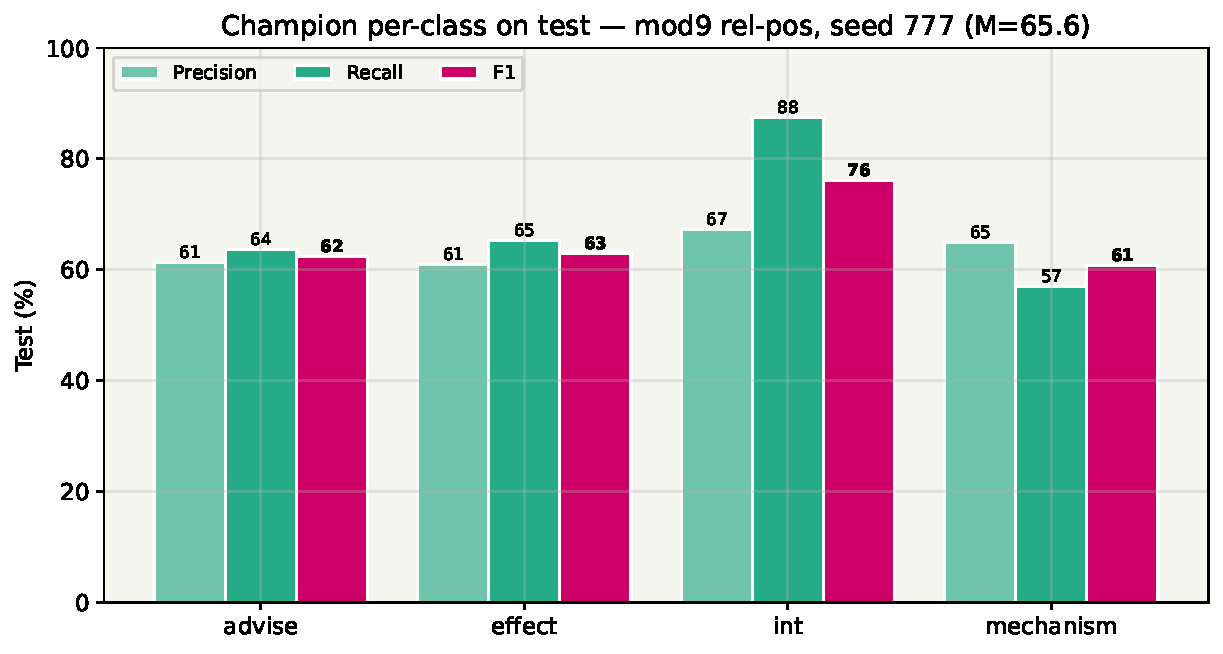
\includegraphics[width=0.6\linewidth]{fig22_per_class_test.pdf}
\caption{System 2.2 champion (\texttt{mod9} rel-pos, seed 777) per-class on test, M-F1 = 65.6. As in 2.1, \texttt{int} is the strongest class (F1 = 76.1, driven by very high recall).}
\label{fig:nn-champ}
\end{figure}

\begin{cmpbox}\small
\textbf{2.2 vs.\ Task~1's BiLSTM.} The two NN systems behave almost
identically methodologically: \emph{input representation} is the
dominant lever (+10\,pp here, $\sim$+9\,pp there), architecture and HP
tweaks are neutral-to-negative, and a \emph{seed audit} is mandatory
because the devel-best seed is a lucky outlier whose test rank is
anti-correlated. The DDI-specific twist is the relative-position
embedding, which has no NER analogue, in NER every token is its own
label, so ``distance to the entity pair'' is meaningless, whereas in DDI
it is the single most useful learned feature.
\end{cmpbox}

\begin{okbox}
\textbf{System 2.2 final: BiLSTM + relative-position embedding,
devel-selected seed 777 $\to$ test M-F1 = 65.6}, within 1.2\,pp of the
ML champion, and reached \emph{without} a single hand-crafted
syntactic feature. The recurring lesson is the same as 2.1:
\emph{representation $>$ architecture $>$ hyperparameters}, and
single-seed peaks must be treated with suspicion.
\end{okbox}

%% ============================================================
\section{System 2.3 - DDI with Large Language Models}\label{sec:llm}
%% ============================================================

System 2.3 asks whether a small, instruction-tuned LLM can match the
dedicated systems, as it did, strikingly, on Task~1's NER. The brief
names three axes: prompt adaptation, few-shot example selection, and
fine-tuning (examples and hyperparameters). We work through all three.

\subsection{Starting point and output format}
The LLM frames DDI as \textbf{single-label generation}: the two target
drugs are masked in the sentence as \texttt{[DRUG1]} / \texttt{[DRUG2]}
(other entities as \texttt{[DRUG\_OTHER]}), and the model is asked to
emit exactly one of the five class labels. We use two
4-bit-quantised 3B instruction models, \textbf{Llama-3.2-3B} and
\textbf{Qwen-2.5-3B}, on the Boada cluster. Note the fundamental
difference from Task~1: there the LLM \emph{generated XML-tagged text}
(a structured-generation task that played to its strengths); here it
emits a \emph{single token}, so it gets none of that structured-output
advantage, a point we return to in the conclusions.

\subsection{Phase~C - few-shot experiments}
We first measured how far prompting alone can go, sweeping the number of
in-context demonstrations $k$.

\begin{table}[H]
\centering\small
\renewcommand{\arraystretch}{1.12}
\rowcolors{2}{accentgrey!30}{white}
\begin{tabular}{>{\bfseries\color{upcblue}}l r r r r r}
\toprule
\rowcolor{upcblue}\textcolor{white}{\textbf{$k$ shots (Llama, p01)}} & \textcolor{white}{0} & \textcolor{white}{3} & \textcolor{white}{5} & \textcolor{white}{10} & \textcolor{white}{15} \\
\midrule
devel macro-F1 & 9.5 & 21.4 & 21.0 & \textbf{23.2} & 21.8 \\
devel micro-F1 & 8.2 & 18.7 & 18.7 & 17.4 & 22.0 \\
\bottomrule
\end{tabular}
\caption{Few-shot $k$-sweep. Performance jumps from near-zero at $k{=}0$ to $\approx$23 at $k{=}10$, then plateaus, more demonstrations do not help. A second prompt template (\texttt{prompts02}) peaked similarly (M=21.8 at $k{=}10$), and Qwen few-shot reached only M=19.8.}
\label{tab:fs}
\end{table}

\begin{figure}[H]
\centering
\begin{subfigure}[t]{0.52\textwidth}
\centering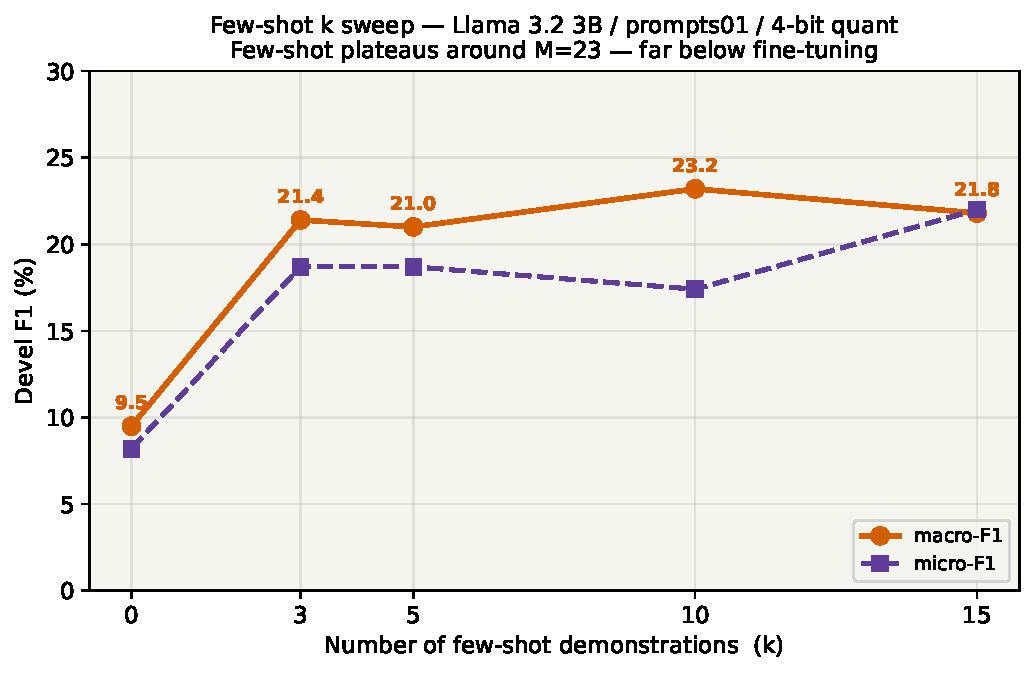
\includegraphics[width=\linewidth]{fig23_fs_sweep.pdf}
\caption{Few-shot $k$-sweep (Llama, \texttt{prompts01}).}
\end{subfigure}\hfill
\begin{subfigure}[t]{0.46\textwidth}
\centering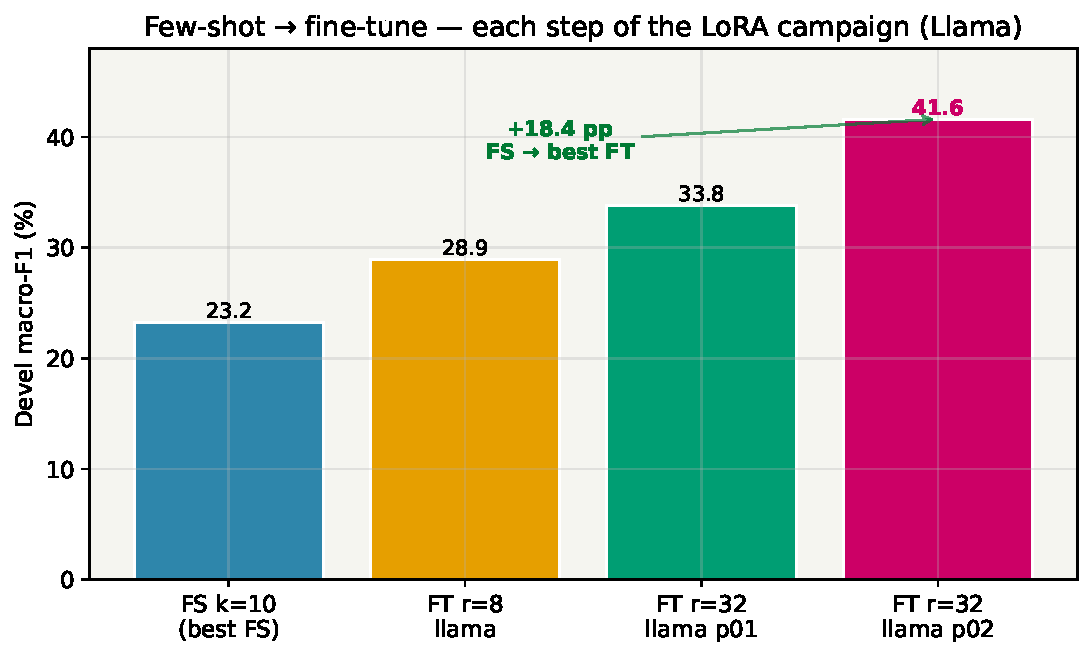
\includegraphics[width=\linewidth]{fig23_fs_vs_ft.pdf}
\caption{Few-shot $\to$ fine-tune jump.}
\end{subfigure}
\caption{Few-shot inference plateaus around macro-F1 = 23 regardless of $k$, far below even the weakest fine-tune. Fine-tuning is essential.}
\label{fig:llm-fs}
\end{figure}

\textbf{Finding: few-shot is not enough for DDI.} At M$\approx$23 the
best few-shot config trails the ML champion by \textbf{$-$44\,pp}. This
is the \emph{first} divergence from Task~1, where few-shot was far more
competitive (best NER few-shot reached test micro-F1 $\approx$49\,\%,
macro $\approx$40\,\%). The relational, imbalanced nature of DDI is much
harder to convey in a handful of in-context examples than the
span-spotting of NER. Fine-tuning is mandatory.

\subsection{Phase~D/F - LoRA fine-tuning: rank, model and prompt}
We fine-tuned both models with LoRA at two ranks ($r{=}8$, $r{=}32$,
$\alpha{=}2r$) and two prompt templates. \texttt{prompts02} fixes a typo
in the \texttt{advise} class definition and strengthens the ``do not
invent an interaction'' instruction for \texttt{null}.

\begin{table}[H]
\centering\small
\renewcommand{\arraystretch}{1.15}
\rowcolors{2}{accentgrey!30}{white}
\begin{tabular}{>{\bfseries\color{upcblue}}l r r r r}
\toprule
\rowcolor{upcblue}\textcolor{white}{\textbf{Fine-tune config}} & \textcolor{white}{\textbf{devel M}} & \textcolor{white}{\textbf{devel m}} & \textcolor{white}{\textbf{test M}} & \textcolor{white}{\textbf{test m}} \\
\midrule
Llama $r{=}8$            & 28.9 & 36.0 & 30.5 & 35.3 \\
Qwen  $r{=}8$            & 33.7 & 33.7 & 27.6 & 29.4 \\
Llama $r{=}32$ p01       & 33.8 & 37.6 & 35.2 & 37.8 \\
Qwen  $r{=}32$ p01       & 32.5 & 34.5 & 29.1 & 32.0 \\
\rowcolor{upclight}\textbf{Llama $r{=}32$ p02} & \textbf{41.6} & \textbf{42.5} & \textbf{39.8} & \textbf{40.9} \\
Qwen  $r{=}32$ p02 (10ep)& 28.8 & 29.2 & 26.0 & 26.8 \\
Qwen  $r{=}32$ p02 (3ep) & 30.9 & 29.9 & 25.9 & 27.0 \\
\bottomrule
\end{tabular}
\caption{All fine-tune configurations. The champion is \textbf{Llama $r{=}32$ / \texttt{prompts02} (test M = 39.8)}. Doubling the LoRA rank and improving the prompt each add $\approx$+5\,pp on Llama.}
\label{tab:ft}
\end{table}

\begin{figure}[H]
\centering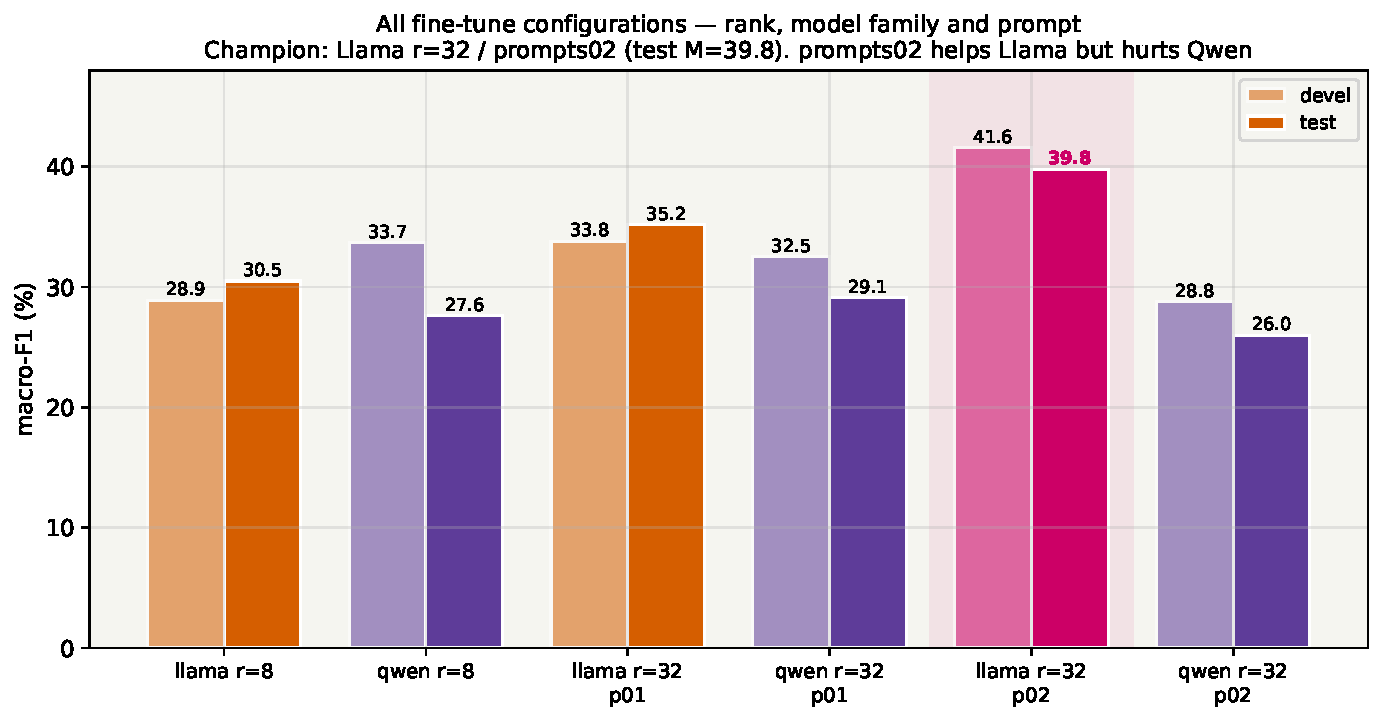
\includegraphics[width=0.95\linewidth]{fig23_ft_configs.pdf}
\caption{All fine-tune configurations (devel + test macro-F1). LoRA rank $8\to32$ and prompt quality are each as powerful as the other, prompt design is a first-class capacity lever, not a free afterthought.}
\label{fig:llm-ft}
\end{figure}

\textbf{Findings.}
\begin{itemize}
    \item \textbf{Fine-tuning closes part of the few-shot gap}, from
    M$\approx$23 to 39.8, but no further: the ceiling is far below
    ML/NN.
    \item \textbf{LoRA rank is a real capacity knob.} $r{=}8\to32$ on
    Llama gives +5\,pp test (30.5$\to$35.2). This is the DDI analogue of
    the rank lever that helped Task~1's LLM most.
    \item \textbf{Prompt quality is as strong as rank.} Swapping
    \texttt{prompts01}$\to$\texttt{prompts02} adds +4.6\,pp test on
    Llama, a one-file change worth as much as doubling the adapter.
\end{itemize}

\subsection{Phase~G - prompt brittleness across model families}
The prompt result above came with a surprise that is, to us, the most
interesting finding of System 2.3.

\begin{figure}[H]
\centering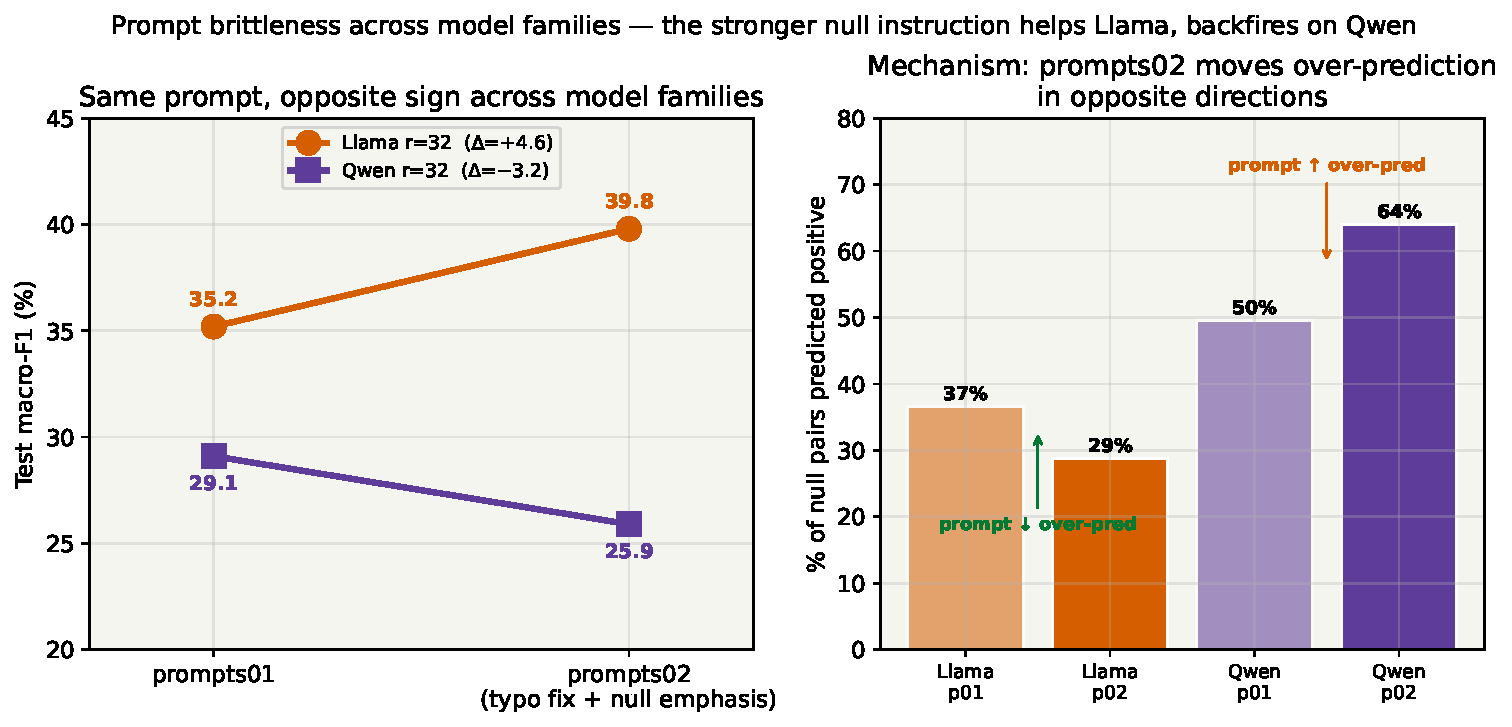
\includegraphics[width=\linewidth]{fig23_prompt_crossmodel.pdf}
\caption{\texttt{prompts02} helps Llama (+4.6\,pp test) but \emph{hurts} Qwen ($-$3.2\,pp). The mechanism (right) is the null over-prediction rate: the stronger \texttt{null} instruction made Llama predict positives \emph{less} (36.6\%$\to$28.8\%) but made Qwen predict them \emph{more} ($\approx$49.6\%$\to$64\%). The same instruction is read as caution by one model and as licence by the other.}
\label{fig:llm-prompt}
\end{figure}

\textbf{Finding: prompt improvements are not transferable across model
families.} The identical prompt that lifts Llama by +4.6\,pp drops Qwen
by $-$3.2\,pp. Llama \emph{follows} the stronger ``do not invent an
interaction'' instruction and over-predicts less; Qwen \emph{over-reacts}
to the richer class definitions and over-predicts more. You cannot tell
which way a prompt will move a given model without running it ,
controllability with a sharp double edge.

\subsection{Phase~H - is the collapse overfitting? An epoch ablation}
Qwen's failure under \texttt{prompts02} could have been overfitting (its
10-epoch run completed fully where Llama's stopped at 3 on a disk
quota). We ran a matched 3-epoch Qwen to remove the confound.

\begin{figure}[H]
\centering
\begin{subfigure}[t]{0.48\textwidth}
\centering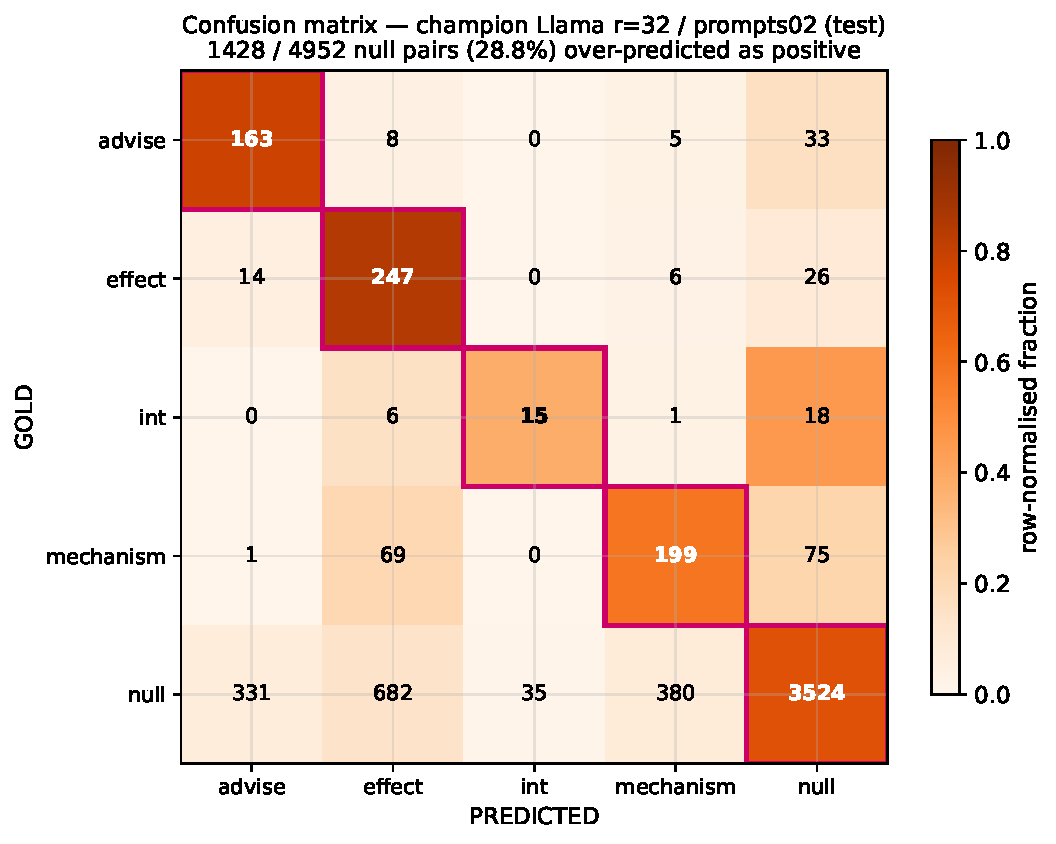
\includegraphics[width=\linewidth]{fig23_confmat.pdf}
\caption{Champion confusion matrix (test).}
\end{subfigure}\hfill
\begin{subfigure}[t]{0.50\textwidth}
\centering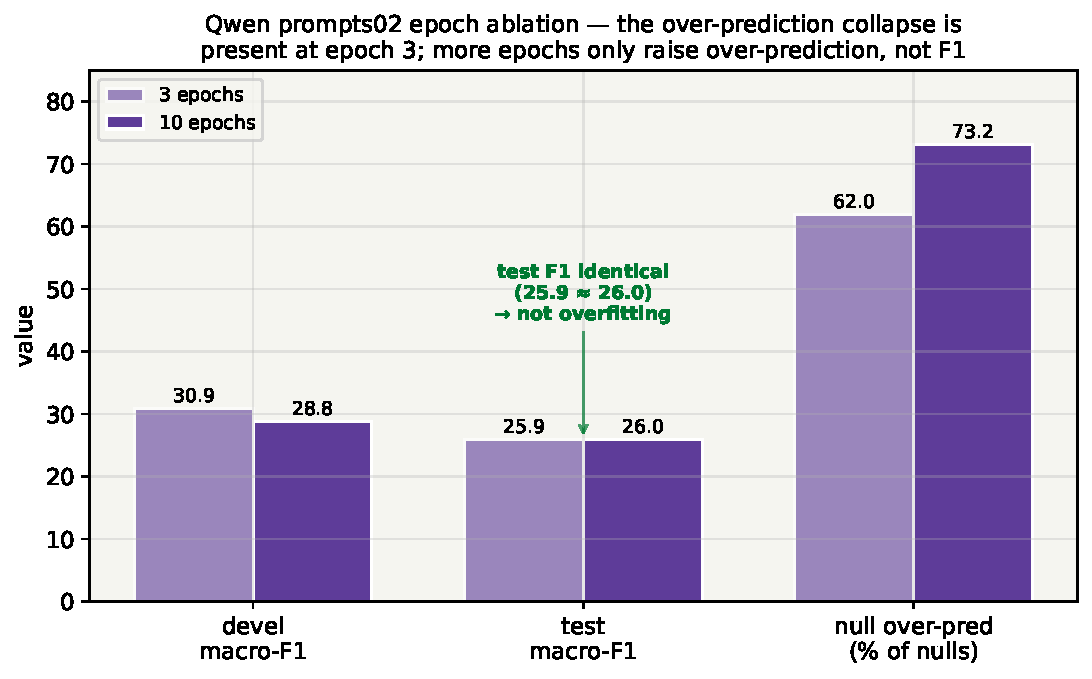
\includegraphics[width=\linewidth]{fig23_epoch_ablation.pdf}
\caption{Qwen \texttt{prompts02}: 3 vs.\ 10 epochs.}
\end{subfigure}
\caption{Left: even the champion over-predicts, 28.8\,\% of all \texttt{null} pairs receive a positive label (precision $\ll$ recall on every class). Right: 3-epoch and 10-epoch Qwen reach \emph{identical} test F1 (25.9 vs 26.0); more epochs only inflate the over-prediction rate (62\%$\to$73\%). The collapse is a property of the model$\times$prompt pairing, not of training length.}
\label{fig:llm-confmat}
\end{figure}

\textbf{Finding: the collapse is not overfitting.} Test F1 is flat
between 3 and 10 epochs; the majority-positive failure mode is locked in
by epoch~3. The confusion matrix of even the \emph{champion} shows the
binding constraint: 1428 / 4952 \texttt{null} pairs (28.8\,\%) are
labelled positive, and recall exceeds precision on every class. The LLM
has not learned \emph{when to abstain}.

\subsection{A negative result: inference-time length filtering}
Because all three systems degrade on long sentences, we tested whether
forcing \texttt{null} on long sentences would help the LLM.

\begin{table}[H]
\centering\small
\renewcommand{\arraystretch}{1.12}
\rowcolors{2}{accentgrey!30}{white}
\begin{tabular}{>{\bfseries\color{upcblue}}l r r r r}
\toprule
\rowcolor{upcblue}\textcolor{white}{\textbf{Filter (test M)}} & \textcolor{white}{\textbf{none}} & \textcolor{white}{\textbf{drop $>$50w}} & \textcolor{white}{\textbf{drop $>$40w}} & \textcolor{white}{\textbf{drop $>$30w}} \\
\midrule
Llama $r{=}32$ p02 & \textbf{39.8} & 39.6 & 39.0 & 38.5 \\
Llama $r{=}32$ p01 & 35.2 & 35.2 & 34.8 & 34.7 \\
\bottomrule
\end{tabular}
\caption{Length-filter post-processing. It never helps and tighter thresholds hurt, because the model already self-suppresses on long sentences (only $\approx$2\,\% of its positive predictions fall in $>$50-word sentences).}
\label{tab:lenfilter}
\end{table}

\begin{figure}[H]
\centering
\begin{subfigure}[t]{0.50\textwidth}
\centering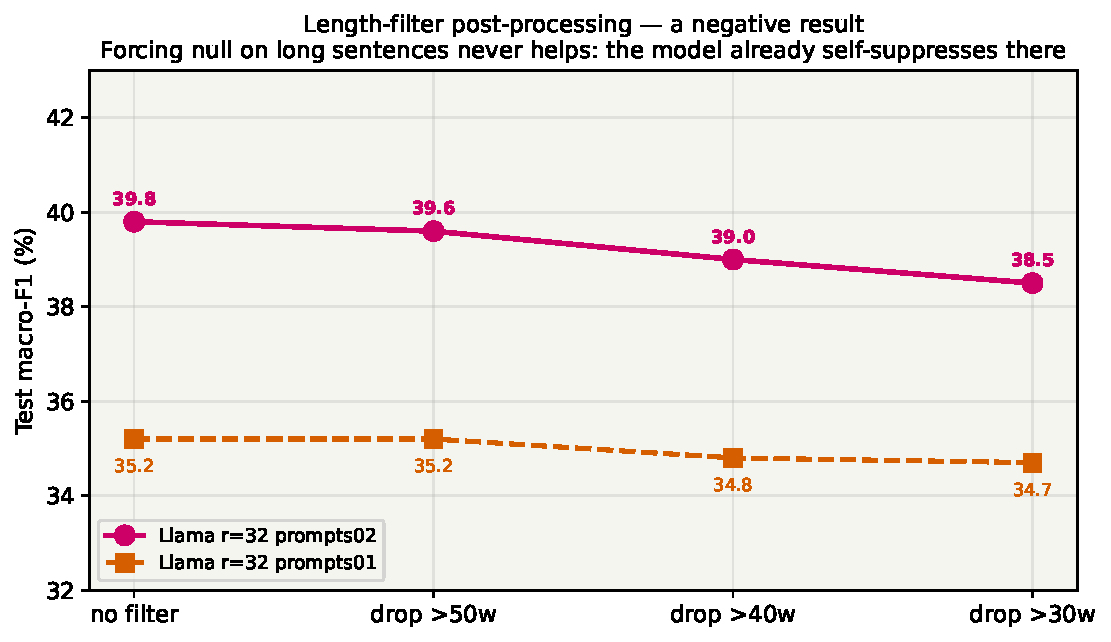
\includegraphics[width=\linewidth]{fig23_length_filter.pdf}
\caption{Length-filter post-processing (negative).}
\end{subfigure}\hfill
\begin{subfigure}[t]{0.48\textwidth}
\centering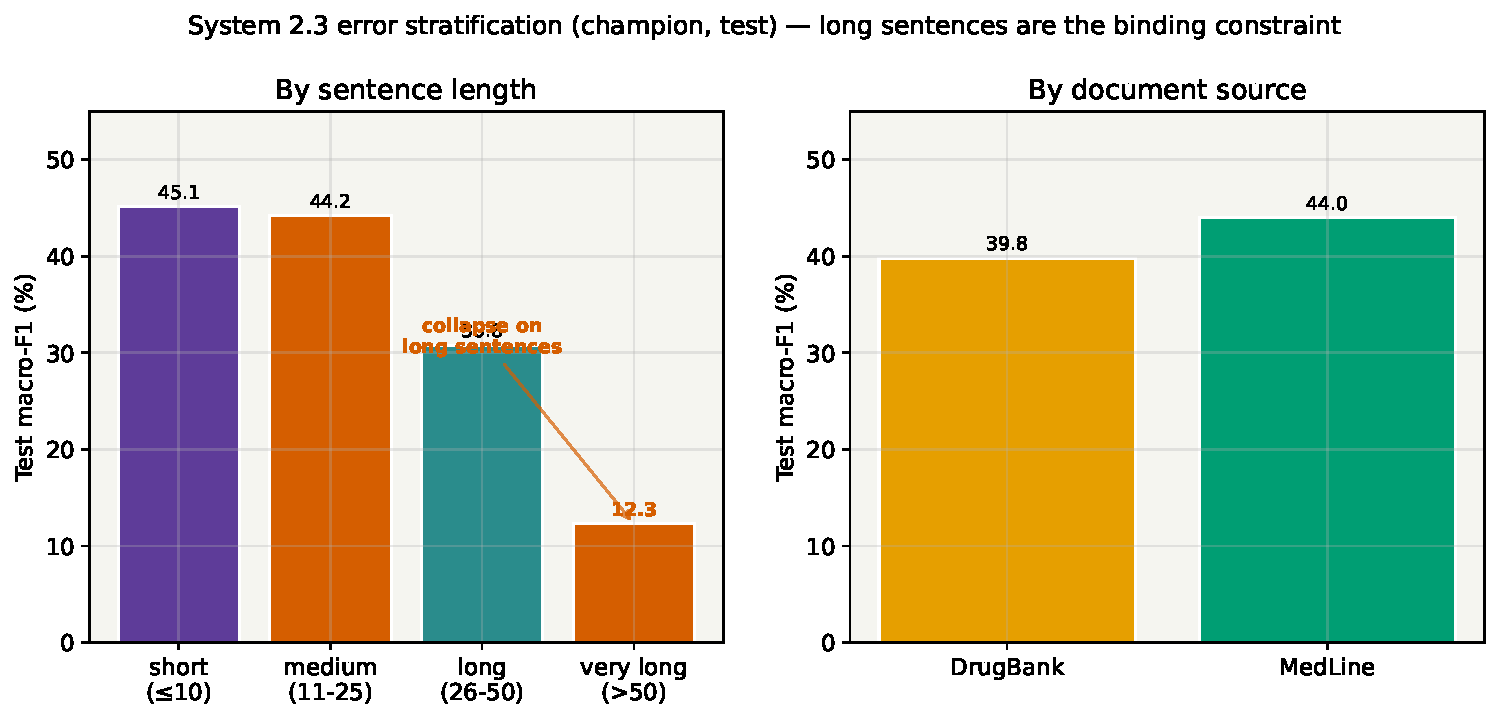
\includegraphics[width=\linewidth]{fig23_strata.pdf}
\caption{Error stratification (champion, test).}
\end{subfigure}
\caption{Left: forcing \texttt{null} on long sentences never helps, the collapse there is a \emph{recall} problem (positives missed), not a precision one a filter could fix. Right: like 2.1 and 2.2, the LLM degrades sharply on long sentences (M = 12.3 on $>$50 words), and MedLine is actually slightly easier than DrugBank for the LLM (the opposite of 2.1).}
\label{fig:llm-neg}
\end{figure}

\textbf{Finding.} The vlong-sentence collapse (M=12.3) cannot be patched
at inference: the model rarely fires there in the first place, so
removing those predictions loses true positives without gaining
precision. The fix would require \emph{more} signal on long sentences
(bigger context window, stronger long-range attention), not less.

\subsection{Discussion and comparison to Task~1}
\begin{cmpbox}\small
\textbf{2.3 vs.\ Task~1's LLM, the central surprise.} The same recipe
(4-bit 3B, LoRA, prompt+rank tuning) \emph{won} macro-F1 on NER
(M=76.3, beating both classical systems) yet \emph{loses} DDI by
$\approx$27\,pp. Three structural reasons, developed in
Section~\ref{sec:conclusions}: DDI is \emph{relational} (the answer is a
property of two entities and the syntax between them, not of one span);
the 85\,\% \texttt{null} imbalance drives systematic over-prediction;
and the single-token output removes the structured-generation advantage
NER handed the LLM. The two transferable wins from NER still hold ,
fine-tuning $\gg$ few-shot, and rank/prompt are the levers, but they
are not enough on this task.
\end{cmpbox}

\begin{okbox}
\textbf{System 2.3 final: LoRA fine-tuned Llama-3.2-3B, $r{=}32$,
\texttt{prompts02} $\to$ test M-F1 = 39.8.} Three findings: (1)
fine-tuning is mandatory, few-shot plateaus 17\,pp lower; (2) prompt
quality is a first-class capacity lever, as strong as LoRA rank, but it
is \textbf{not transferable across model families}; (3) the binding
constraint is the positive/\texttt{null} boundary, the model
over-predicts interactions and no inference-time guardrail repairs it.
\end{okbox}

%% ============================================================
\section{Conclusions: Cross-System Comparison}\label{sec:conclusions}
%% ============================================================

All three systems attack the \emph{same} DDI task and are scored by the
\emph{same} evaluator on the \emph{same} test split, so the numbers are
directly comparable, and comparable in turn to Task~1, which used the
identical protocol on the NER half of the corpus.

\subsection{Headline test-set results}

\begin{figure}[H]
\centering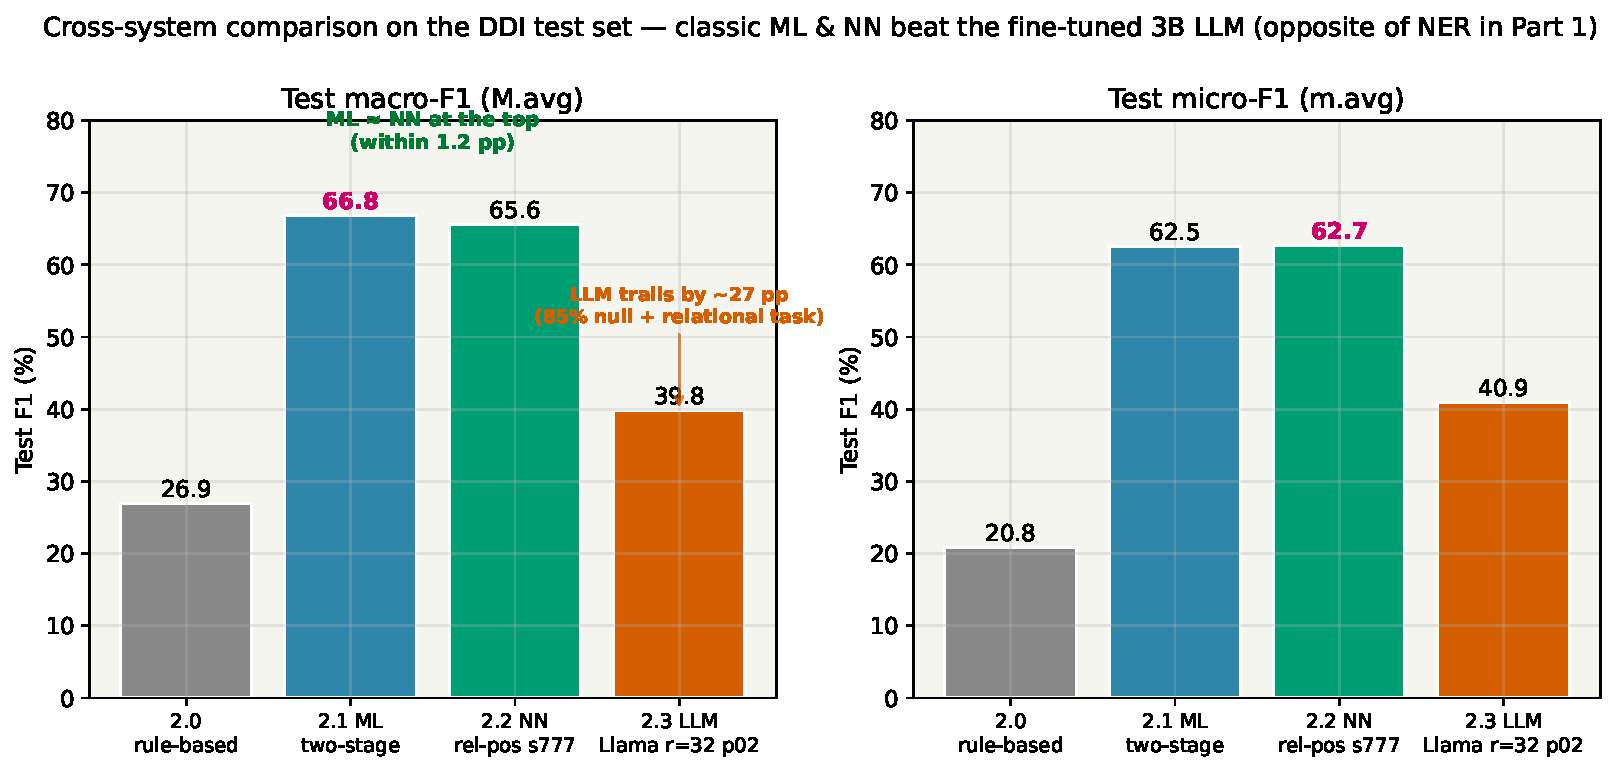
\includegraphics[width=\linewidth]{fig2_cross_system.pdf}
\caption{Cross-system test F1. The classical ML system wins macro-F1 (66.8), the neural network is within 1.2\,pp (65.6), and the fine-tuned 3B LLM trails both by $\approx$27\,pp (39.8). This is the \emph{mirror image} of Task~1 (NERC), where the fine-tuned LLM won macro-F1 outright.}
\label{fig:cross}
\end{figure}

\begin{table}[H]
\centering\small
\renewcommand{\arraystretch}{1.2}
\rowcolors{2}{accentgrey!30}{white}
\begin{tabular}{>{\bfseries\color{upcblue}}l r r r r r r}
\toprule
\rowcolor{upcblue}\textcolor{white}{\textbf{System (test)}} & \textcolor{white}{\textbf{M-F1}} & \textcolor{white}{\textbf{m-F1}} & \textcolor{white}{\textbf{advise}} & \textcolor{white}{\textbf{effect}} & \textcolor{white}{\textbf{int}} & \textcolor{white}{\textbf{mech.}} \\
\midrule
2.0 rule-based                 & 26.9 & 20.8 & 20.1 & 25.2 & 50.0 & 12.3 \\
\textbf{2.1 ML (two-stage)}    & \cellcolor{upclight}\textbf{66.8} & 62.5 & \textbf{64.8} & 63.0 & \textbf{80.0} & 59.3 \\
2.2 NN (rel-pos, seed 777)     & 65.6 & \textbf{62.7} & 62.4 & 63.0 & 76.1 & \textbf{60.7} \\
2.3 LLM (Llama $r{=}32$ p02)   & 39.8 & 40.9 & 45.4 & 37.9 & 33.3 & 42.6 \\
\bottomrule
\end{tabular}
\caption{Headline test-set comparison (\% F1; best positive-class values in bold). ML and NN are effectively a tie at the top; the LLM trails on every class and is weakest on the rare \texttt{int}.}
\label{tab:cross}
\end{table}

\begin{figure}[H]
\centering
\begin{subfigure}[t]{0.62\textwidth}
\centering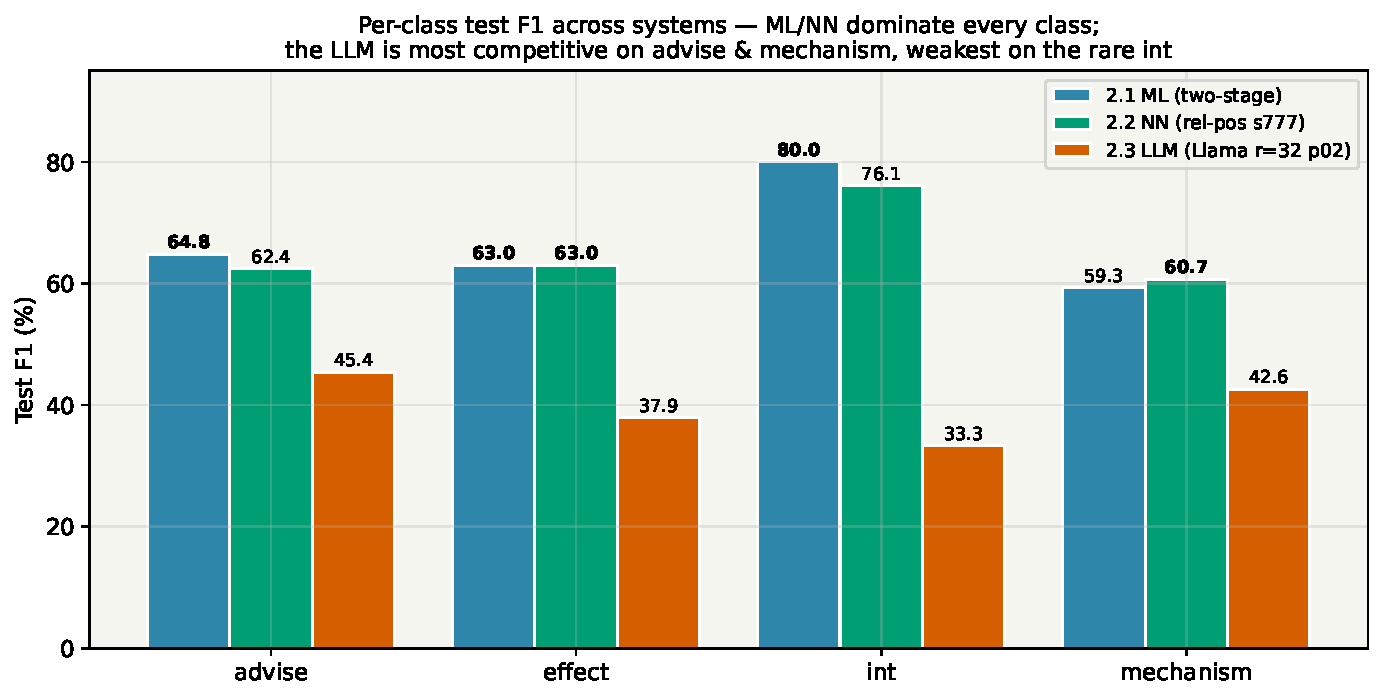
\includegraphics[width=\linewidth]{fig2_cross_perclass.pdf}
\caption{Per-class test F1 across systems.}
\end{subfigure}\hfill
\begin{subfigure}[t]{0.36\textwidth}
\centering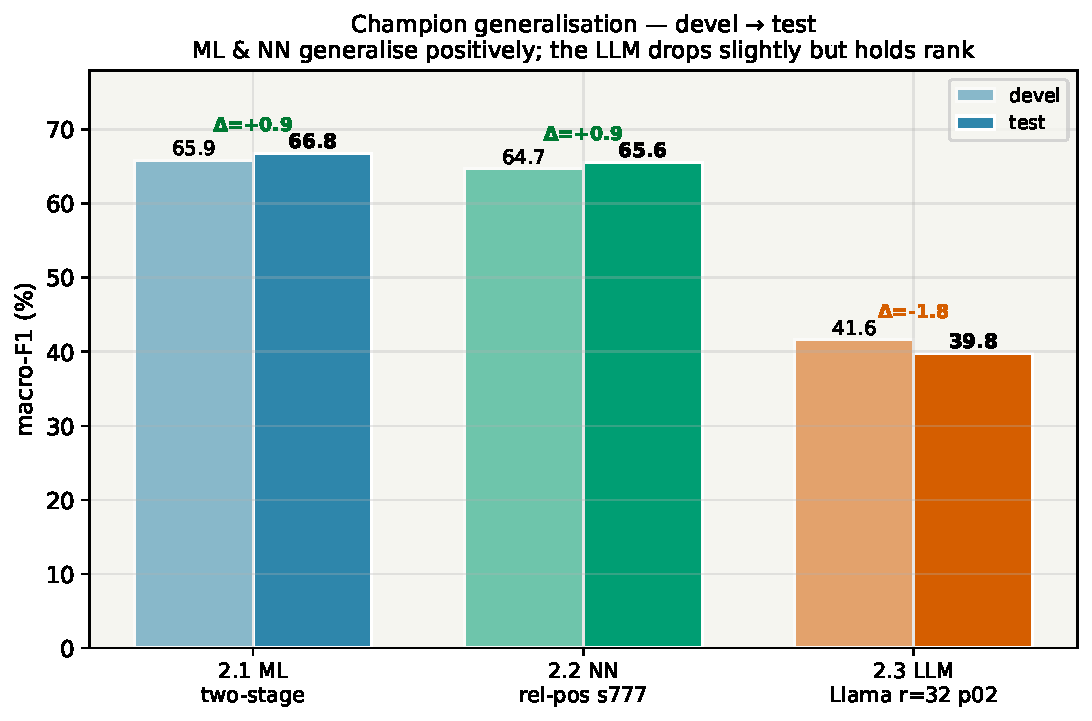
\includegraphics[width=\linewidth]{fig2_cross_devtest.pdf}
\caption{Champion devel$\to$test generalisation.}
\end{subfigure}
\caption{ML and NN dominate every class; the LLM is most competitive on \texttt{advise} and \texttt{mechanism} and weakest on the rare \texttt{int}. All three champions generalise sensibly from devel to test.}
\label{fig:cross2}
\end{figure}

\subsection{Trade-offs: effort, cost, explainability, controllability, performance}
The brief asks explicitly for a comparison across these five dimensions.

\begin{itemize}
\item \textbf{Development effort.} 2.1 required the most \emph{thinking}
(feature engineering, the solver sweep, the two-stage decomposition) but
each idea is a few lines and a 3-minute re-run. 2.2 was moderate (four
input channels, the relative-position embedding, architecture flags).
2.3 was the \emph{least code} (env-var knobs for LoRA rank and epochs, a
second prompt file) but the longest \emph{wall-clock} per idea by far.
\item \textbf{Computational cost.} 2.1 runs entirely on CPU: feature
extraction $\approx$3\,min, training in seconds, the whole campaign
is minutes. 2.2 trains in $\approx$5--15\,min per seed on one GPU
($\approx$1\,h for a 5-seed audit). 2.3 is \textbf{two orders of
magnitude} more expensive: a single fine-tune is 1.5--5.4\,GPU-hours and
inference alone runs up to $\approx$5\,GPU-hours for Qwen; the full LLM
campaign consumed tens of GPU-hours and repeatedly hit the cluster's
2\,GB disk quota.
\item \textbf{Explainability.} 2.1 is the most interpretable: the
learned feature weights are directly inspectable (\texttt{same-drug} is
the model's strongest signal; class-appropriate trigger verbs follow),
and every mod's effect has a concrete cause. 2.2 is intermediate
(input-channel ablations are interpretable; hidden states are not). 2.3
is the least: we can \emph{observe} that Qwen over-predicts under
\texttt{prompts02} but cannot point to why inside a 3B network.
\item \textbf{Controllability.} 2.3 offers the most direct behavioural
handles at inference (a one-line prompt swap visibly reshapes per-class
recall), but those handles are \textbf{brittle and non-transferable},
as the opposite Llama/Qwen prompt response shows. 2.1 is controllable
through its feature set and a single smooth stage-1 threshold (a
predictable precision/recall dial); 2.2 only through architecture flags
fixed at training time.
\item \textbf{Performance.} On this task the ordering is unambiguous:
\textbf{2.1 ML (66.8) $\approx$ 2.2 NN (65.6) $\gg$ 2.3 LLM (39.8)} on
macro-F1. The classical pipeline wins.
\end{itemize}

\begin{table}[H]
\centering\small
\renewcommand{\arraystretch}{1.25}
\rowcolors{2}{accentgrey!30}{white}
\begin{tabular}{>{\bfseries\color{upcblue}}l c c c}
\toprule
\rowcolor{upcblue}\textcolor{white}{\textbf{Dimension}} & \textcolor{white}{\textbf{2.1 ML}} & \textcolor{white}{\textbf{2.2 NN}} & \textcolor{white}{\textbf{2.3 LLM}} \\
\midrule
Test macro-F1                & \textbf{66.8} & 65.6 & 39.8 \\
Compute per experiment       & seconds (CPU) & $\sim$10\,min (GPU) & 2--10\,h (GPU) \\
Development effort           & feature design & moderate & least code \\
Explainability               & \yes\ high & \partialmark\ partial & \no\ low \\
Controllability              & threshold dial & training-time only & prompt (brittle) \\
\bottomrule
\end{tabular}
\caption{Five-axis comparison the brief asks for. On DDI, the classical pipeline dominates on performance, cost \emph{and} explainability; the LLM's only edge is natural-language controllability, which proved brittle.}
\label{tab:tradeoffs}
\end{table}

\subsection{Why the LLM loses on DDI but won on NERC}
\begin{warnbox}\small
The same 3B LoRA recipe \emph{won} macro-F1 on Task~1 (NER: M=76.3, vs
69.1 BiLSTM and 68.2 CRF) yet trails by $\approx$27\,pp here. Three
structural reasons explain the reversal:
\textbf{(1) the task is relational}, not a surface property of one span
, the answer depends on the syntactic relationship between two marked
drugs, which 2.1 encodes explicitly via dependency-path features and the
LLM must reconstruct from raw text;
\textbf{(2) the 85\,\% \texttt{null} imbalance} drives the LLM into
systematic over-prediction (it labels $\approx$29--64\,\% of true
\texttt{null} pairs as positive), the single largest error source ,
NER had no equivalent ``null pair'' notion;
\textbf{(3) the output is a single token}, so the LLM gets none of the
structured-generation advantage that helped it spot rare entities on the
span-tagging NER task. None of these is fixable by prompting at the
3B/4-bit scale our hardware allows.
\end{warnbox}

\subsection{When is each system the right choice?}
\begin{itemize}
\item \textbf{Use 2.1 (ML)} as the default for DDI: best macro-F1,
CPU-only, fully interpretable, minutes per iteration. On a relational,
syntax-driven task with hand-crafted dependency features, classical ML
is hard to beat.
\item \textbf{Use 2.2 (NN)} when a GPU is available and one prefers
learned representations to feature engineering; it reaches within 1.2\,pp
of ML \emph{without} any hand-crafted syntactic features, and the
relative-position embedding is the key to getting there.
\item \textbf{Use 2.3 (LLM)} only where its flexibility (zero feature
engineering, natural-language control) outweighs a large accuracy and
cost penalty. At 3B/4-bit it is not competitive for DDI; a larger,
full-precision model might narrow the gap but would not change the
ranking on this hardware.
\end{itemize}

\paragraph{Overall conclusion.}
For DDI-2013 the three paradigms finish \textbf{2.1 ML = 66.8\,\%},
\textbf{2.2 NN = 65.6\,\%}, \textbf{2.3 LLM = 39.8\,\%} macro-F1. The
central, task-independent lesson, consistent with Task~1, is that
\textbf{representation matters more than architecture}: in 2.1 a feature
\emph{combination} plus the two-stage decomposition delivered the gains,
in 2.2 the input channels and the relative-position embedding did, and
in 2.3 the LoRA rank and the prompt did. But the headline lesson of
Task~2 is the \emph{contrast} with NER: a small fine-tuned LLM can match
dedicated systems on a span-extraction task, yet on a \emph{relational}
task with heavy class imbalance and a syntactic signal, the classical
feature-based pipeline remains clearly ahead, the right tool depends
on the shape of the task, not on the recency of the technique.

\end{document}
